\documentclass[11pt]{article}

\usepackage[letterpaper,margin=1in]{geometry}
\usepackage[T1]{fontenc}
\usepackage[utf8]{inputenc}
\usepackage{amsmath,amssymb,amsfonts,stmaryrd,mathtools}
\usepackage{amsthm}
\usepackage{mathpartir}
\usepackage{enumitem}
\usepackage{booktabs}
\usepackage{listings}
\usepackage{xcolor}
\usepackage{tikz}
\usepackage[expansion=false]{microtype}
\usepackage[hidelinks]{hyperref}

\usetikzlibrary{arrows.meta,positioning,fit,backgrounds,calc}

% ---------- theorem environments ----------
\theoremstyle{definition}
\newtheorem{definition}{Definition}[section]
\newtheorem{example}[definition]{Example}
\newtheorem{construction}[definition]{Construction}
\theoremstyle{plain}
\newtheorem{theorem}[definition]{Theorem}
\newtheorem{lemma}[definition]{Lemma}
\newtheorem{proposition}[definition]{Proposition}
\newtheorem{corollary}[definition]{Corollary}
\theoremstyle{remark}
\newtheorem{remark}[definition]{Remark}
\newtheorem{nonexample}[definition]{Non-example}

% ---------- notation ----------
\newcommand{\GSLT}{\mathbf{GSLT}}
\newcommand{\iGSLT}{\mathbf{iGSLT}}
\newcommand{\ciGSLT}{\mathbf{ciGSLT}}
\newcommand{\Lcat}{\mathbf{L}}
\renewcommand{\Pr}{\mathrm{Pr}}
\newcommand{\Nm}{\mathrm{Nm}}
\newcommand{\Sig}{\mathsf{Sig}}
\newcommand{\Stk}{\mathsf{Stk}}
\newcommand{\Surf}{\mathsf{Surf}}
\newcommand{\Tw}{\mathsf{T}}
\newcommand{\cost}{\mathcal{C}}
\newcommand{\hist}{\mathcal{H}}
\newcommand{\hyp}{\mathcal{K}}
\newcommand{\rsq}{\rightsquigarrow}
\newcommand{\compute}{\mathrm{compute}}
\newcommand{\near}{\mathrm{near}}
\newcommand{\cf}{\mathrm{cf}}
\newcommand{\sem}[1]{\llbracket #1 \rrbracket}
\newcommand{\angles}[3]{\langle #1 \rangle_{#2}\,#3}
\newcommand{\fv}{\mathrm{FV}}
\newcommand{\Zc}{\mathcal{Z}}
\newcommand{\ctxbar}{\,|\,}

% ---------- listings ----------
\definecolor{kwcol}{rgb}{0.20,0.20,0.65}
\definecolor{strcol}{rgb}{0.60,0.20,0.15}
\definecolor{comcol}{rgb}{0.40,0.45,0.40}

\lstdefinestyle{mettail}{
  basicstyle=\ttfamily\footnotesize,
  keywordstyle=\color{kwcol}\bfseries,
  stringstyle=\color{strcol},
  commentstyle=\color{comcol}\itshape,
  morekeywords={language,types,terms,equations,rewrites,literals,name,for,new,contract,match,where,in,select},
  morecomment=[l]{//},
  morestring=[b]",
  showstringspaces=false,
  columns=fullflexible,
  keepspaces=true,
  breaklines=true,
  frame=leftline,
  framesep=6pt,
  xleftmargin=10pt,
  aboveskip=8pt,
  belowskip=8pt,
}
\lstset{style=mettail}

\title{\bf Graph-Structured Lambda Theories\\[2mm]
\large A Reference for the Working Developer}
\author{}
\date{Draft --- \today}

\begin{document}
\maketitle

\begin{abstract}
A graph-structured lambda theory (GSLT) is a language presentation: a lambda theory ---
so that terms carry variables --- together with a set of equations and an adjoined graph
of rewrite rules. This document is a
reference account of what can be built once a language is presented that way. We
develop the definition and two successive strengthenings --- \emph{interactive} GSLTs,
which name a site of interaction, and \emph{continued} interactive GSLTs, whose
interaction is presented as a meterable cut --- and we discriminate the two with
worked examples, including examples that fail. We then assemble the category $\GSLT$,
whose morphisms preserve bisimulation over context-labelled transitions, and exhibit
three constructions on it: the cost monad $\cost$, which meters a theory; the history
monad $\hist$, which logs it; and the Hypercube functor, a member of the OSLF family of
algorithms, which generates a family of type systems from the theory's own rewrite
rules. Finally we show that all of this is programmable. The \texttt{language!} block of
Rholang~1.4 is a data definition language whose data can wiggle: without equations or
rewrites it presents algebraic data types, with equations it presents finitely
presentable universal algebra, and with rewrites it presents domain-specific languages.
The control flow language is a Rholang whose channels are typed by such specifications,
and whose \texttt{for}-comprehension carries a \texttt{where} clause guarding
communication on context-labelled modal formulae drawn from the generated logic.
\end{abstract}

\tableofcontents

\clearpage

%===============================================================================
\section{Introduction}
%===============================================================================

\subsection{The claim}

A language is a triple. A lambda theory says what can be written, and says it in a term
language with variables; equations say which writings are the same; an adjoined graph of
rewrites says how writings move. Everything this document
develops --- a type system, a cost discipline, a history log, a runtime, a logic for
stating properties of programs --- is generated from that triple, and generated
uniformly, by constructions that do not know which language they are applied to.

That is an ambitious claim and it is worth saying immediately what it does not mean. It
does not mean that every interesting question about a language is answered by its
presentation; it means that a surprising number of the artifacts we are used to
building by hand, once per language, are functorial in the presentation. The cost of
adding cost accounting to a new calculus should not be a research programme. The cost
of getting a type system for a new domain-specific language should not be a semester.
If the presentation is the input, these become instances of one construction rather
than a series of fresh inventions.

\subsection{Who this is for}

Two audiences, addressed simultaneously and, we hope, without either being short-changed.

The first is the reader who wants the mathematics. We assume a working knowledge of
category theory --- categories, functors, adjunctions, monads, and enough fibrational
language to read a subobject fibration without alarm --- and we state the constructions
at the level of generality at which they are true.

The second is the reader who wants to ship something. Every construction in this
document is accompanied by a specification that a machine accepts. Where we say that a
calculus is a GSLT, we give the \texttt{language!} block that presents it. Where we say
a property is checkable, we give the syntax in which one writes the check. The formal
sections and the programmable sections are not two treatments of one subject; they are
one treatment, and the reader who skips either will find the other incomplete.

\subsection{Roadmap}

Part~I develops the objects. Section~\ref{sec:gslt} places the definition in the
lineage of structured operational semantics, reads the two halves of the name --- why a
lambda theory and not a Lawvere theory, why an adjoined graph and not an enrichment ---
and climbs a three-rung ladder from algebraic data types through universal algebra to
domain-specific languages.
Section~\ref{sec:interactive} adds the interaction constructor and the interaction cut,
and discriminates the resulting notion with three machines that fail to be instances of
it. Section~\ref{sec:continued} adds the section and the wrappability condition, and
tabulates how each of our running examples does or does not qualify.

Part~II assembles the category. Section~\ref{sec:category} shows why the obvious
definition of a morphism does not survive contact with the canonical encodings, and
rebuilds it with contexts as the primary structure.

Part~III exhibits three constructions on that category:
the cost monad in Section~\ref{sec:cost}, the history monad in Section~\ref{sec:history},
and the generation of type systems in Section~\ref{sec:hypercube}.

Part~IV is the implementation. Section~\ref{sec:rholang} presents Rholang~1.4 as a data
definition language and a control flow language, and reduces the running examples to
specifications a machine accepts.

%===============================================================================
\part*{Part I --- Objects}
\addcontentsline{toc}{part}{Part I --- Objects}
%===============================================================================

\section{Graph-structured lambda theories}
\label{sec:gslt}

\subsection{The lineage: structured operational semantics}

The presentation style we depend on is Plotkin's~\cite{Plotkin1981,Plotkin2004}. Before
structured operational semantics, giving the meaning of a programming construct meant
either a denotational assignment into a domain or an informal appeal to an abstract
machine. Plotkin's proposal was that one could give the behaviour of a language
\emph{syntactically}, by inference rules over the term structure, with the rules for a
compound term given in terms of the rules for its parts. The presentation was finite,
it was checkable, and --- this is the part that matters here --- it was
\emph{structural}: the shape of the rules followed the shape of the grammar.

Milner's \emph{Functions as Processes}~\cite{Milner1992} adopts this style and sets the
standard by which such presentations should be judged. The paper gives the
$\pi$-calculus by a grammar, a structural congruence, and a small family of reduction
rules, and then encodes the $\lambda$-calculus into it. What makes the presentation
exemplary is not merely that it is correct but that it is \emph{complete in the
relevant sense}: the grammar, the congruence, and the rules together are the whole of
the definition. Nothing is left to the reader's operational imagination. One can
mechanically check a claimed reduction, and one can mechanically check that an encoding
respects reduction, because there is nothing to the language beyond what has been
written down.

Cardelli and Gordon's presentation of the mobile ambient
calculus~\cite{CardelliGordon2000} adopts precisely this style, and it is instructive
to see how little has to change. The ambient calculus is a very different theory ---
its reductions restructure a spatial hierarchy rather than substitute a value --- and
yet the presentation is recognisably the same document: sorts, term formers, a
structural congruence, a handful of reduction rules, and congruence rules closing
reduction under the term formers. The style is not an artifact of process calculi. It
is a general format for presenting a language.

The observation on which this document rests is that once a presentation is
\emph{that} regular, it is data. A grammar is a signature. A structural congruence is a
set of equations. Reduction rules and congruence rules are a set of rewrites. These are
not analogies; they are the same information under different typography. A GSLT is what
you get when you stop treating an SOS presentation as a document to be read by a human
implementer and start treating it as a structure to be consumed by a machine.

\subsection{The definition}

\begin{definition}[Graph-structured lambda theory]
\label{def:gslt}
A \textbf{graph-structured lambda theory} is a triple $G = (\Sigma, E, R)$ consisting of
\begin{itemize}[leftmargin=2em]
  \item a signature $\Sigma$, which is in general a \emph{lambda theory} --- so that
    terms may contain variables;
  \item a set $E$ of equations, imposing a structural congruence $\equiv$; and
  \item a set $R$ of rewrite rules.
\end{itemize}
\end{definition}

The definition is deliberately thin in one direction and deliberately generous in
another, and both deserve comment.

It is thin in that a GSLT is any rewrite theory whatever. Nothing in
Definition~\ref{def:gslt} says the theory is about computation, or that it has processes,
or that anything interacts with anything. The strengthenings of
Sections~\ref{sec:interactive} and~\ref{sec:continued} add exactly the structure later
constructions require, and the discipline of the present document is to add it only when
a construction needs it.\footnote{We say \emph{strengthening} rather than
\emph{enrichment} throughout, reserving the latter for its technical sense, which
Section~\ref{subsec:name} argues is not the right technique here.}

It is generous in that $\Sigma$ is a lambda theory rather than a bare algebraic
signature. That is the substantive choice in the definition, and the next subsection is
about why it was made.

\subsection{Reading the name}
\label{subsec:name}

The two halves of ``graph-structured lambda theory'' are doing two separable jobs. The
\emph{lambda theory} captures the term language --- specifically, a term language
\emph{with variables}. The adjective \emph{graph-structured} captures the rewrite rules.
It is worth taking these in turn, and worth recording the route not taken, because the
route not taken is the one a reader familiar with categorical algebra will expect.

\subsubsection{Why lambda theories and not Lawvere theories}

The natural first thought is that a language presentation is an algebraic theory, and
that the right categorical home for an algebraic theory is a Lawvere
theory~\cite{Lawvere1963}: a category with finite products whose objects are the powers
of a generic object, in which an $n$-ary operation is a morphism $n \to 1$. This is a
beautiful and well-understood setting, and it is not adequate here.

The reason is variables. A Lawvere theory does not generate a term language with
variables; it generates a term language in which variables have been \emph{absorbed into
arities}. A term in $n$ variables is not a term containing variables, it is a morphism
out of $n$. That encoding is faithful for first-order algebra and it breaks down exactly
where we need it not to: one cannot abstract, one cannot have a variable that ranges over
functions, and one cannot write a binder. Every calculus this document treats has
binders --- $\lambda x.M$, $\mathrm{for}(x \leftarrow n)P$, $\mathrm{new}(x, P)$ --- and
a formalism that cannot express a binder cannot present them.

Lambda theories do generate term languages with variables. And in the limit --- that is,
in how the variables get used, which is to say abstraction and application --- lambda
theories are cartesian closed categories. This is the content of the
Curry--Howard--Lambek correspondence~\cite{LambekScott1986}, and it is why the
classifying form of Section~\ref{subsec:classifying} carries a chosen cartesian closed
structure. The CCC structure is not an extra assumption bolted on for the convenience of
Section~\ref{sec:hypercube}; it is what a lambda theory becomes when one asks what its
variables are for.

\subsubsection{Why adjoined and not enriched}

The second natural thought concerns the rewrites. Rewriting looks like $2$-dimensional
structure --- between two terms there is not merely the question of whether they are
equal but a collection of ways of getting from one to the other --- and the standard
technique for such structure is \emph{enrichment}: take hom-objects in the category of
graphs rather than in $\mathbf{Set}$. Graph-enriched Lawvere theories were the initial
approach, and they too are not adequate here.

The difficulty is that enrichment puts the rewrite structure in the wrong place. Under
enrichment the graph of rewrites lives in the hom, where it is available to whatever
respects composition and to nothing else. But we want to \emph{quantify over} rewrites:
the history monad of Section~\ref{sec:history} makes rewrite events into terms, and the
type-generation of Section~\ref{sec:hypercube} reads a rewrite rule together with a
choice of position inside its left-hand side. Neither operation is available to a
construction that can only see hom-objects.

The approach we take instead is to \emph{adjoin} the graph structure to the theory,
as a Lawvere theory of graphs. One says what the sources and the targets are, and ensures
that the source and target maps enjoy the minimal requisite equations. The rewrite
structure thereby becomes ordinary algebraic structure inside the theory, presented by
the same mechanism that presents everything else --- rather than a change of base for
enrichment, sitting outside the theory and constraining it from without. The framing of
operational semantics in this algebraic style follows Stay and
Meredith~\cite{StayMeredith2016} and Baez and Williams~\cite{BaezWilliams2020}.

\begin{remark}[The name, in a nutshell]
\label{rem:nutshell}
\emph{Lambda theory} captures term languages with variables. \emph{Graph-structured}
captures the rewrite rules. A GSLT is a term language with variables, together with an
adjoined graph of rewrites over it.
\end{remark}

\begin{remark}[Why this matters to the reader who wants to ship]
The choice is visible in the specification format. Because the graph structure is
adjoined rather than enriched, the \texttt{rewrites} block of a specification is not a
different \emph{kind} of declaration from the \texttt{terms} block --- it is more
algebraic structure over the same signature. That is why the ladder of
Section~\ref{subsec:ladder} is a ladder rather than three unrelated facilities, and why a
tool that can read the first two blocks can read the third.
\end{remark}

\subsection{Presentation and classifying theory}
\label{subsec:classifying}

Definition~\ref{def:gslt} is syntactic: it is what a developer writes and what a machine
accepts. Several constructions below are more naturally stated semantically, and
Section~\ref{subsec:name} has already said what the semantic form is. We record it
explicitly.

The \emph{classifying theory} of a presentation is a category $\mathsf{T}$ with finite
limits and a chosen cartesian closed structure --- the cartesian closure being what the
lambda theory $\Sigma$ becomes in the limit --- equipped with its subobject fibration
$\pi : \mathrm{Sub}(\mathsf{T}) \to \mathsf{T}$, a distinguished object $\Pr$ of
programs, and a distinguished subobject
\[
  (\rsq) \rightarrowtail \Pr \times \Pr
\]
of one-step reduction, together with entailments generating the base rewrites and their
closure under the term formers. This is the presentation-independent form in which the
type-theoretic construction of Section~\ref{sec:hypercube} takes its input.

The subobject $(\rsq)$ is the adjoined graph of Section~\ref{subsec:name} seen
semantically: its source and target maps are the two projections, and the entailments
generating the base rewrites and closing them under the term formers are the minimal
equations those maps must satisfy. So the two presentations are not two objects to be
reconciled; they are the syntactic and semantic faces of the same construction, and the
reason the classifying theory has exactly the structure it has is that $\Sigma$ is a
lambda theory and $R$ is adjoined as a graph.

We take the presentation as primary throughout, for the practical reason that it is what
one can type, and use the classifying theory when a construction is more naturally stated
in the internal language.

\subsection{The ladder}
\label{subsec:ladder}

Definition~\ref{def:gslt} has three components, and the reader can switch two of them
off. Doing so produces a ladder of three rungs, each of which is a familiar and
independently useful thing. We climb it because it is the most efficient route we know
from ``I already know what this is'' to ``I did not know you could do that.''

\begin{center}
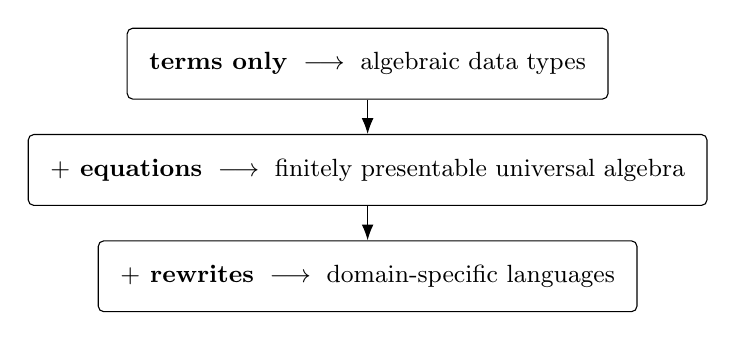
\begin{tikzpicture}[
  rung/.style={draw,rounded corners=2pt,minimum height=9mm,inner xsep=8pt,align=left},
  every node/.style={font=\small}
]
  \node[rung] (r1) at (0,0)
    {\textbf{terms only} \;$\longrightarrow$\; algebraic data types};
  \node[rung] (r2) at (0,-1.35)
    {\textbf{$+$ equations} \;$\longrightarrow$\; finitely presentable universal algebra};
  \node[rung] (r3) at (0,-2.7)
    {\textbf{$+$ rewrites} \;$\longrightarrow$\; domain-specific languages};
  \draw[-{Latex[length=2mm]}] (r1) -- (r2);
  \draw[-{Latex[length=2mm]}] (r2) -- (r3);
\end{tikzpicture}
\end{center}

\subsubsection{Rung one: terms only}

Take $E = \emptyset$ and $R = \emptyset$. What remains is a multi-sorted signature: a
set of sorts and a set of operators with declared argument sorts and result sort. The
terms over such a signature, up to nothing at all, are exactly the inhabitants of an
algebraic data type.

\begin{lstlisting}
language! {
    name: Json,

    types {
        Value
        Field
    },

    terms {
        JNull  . Value ::= "null" ;
        JBool  . b:Bool |- b : Value ;
        JNum   . n:BigRat |- n : Value ;
        JStr   . s:Str |- s : Value ;
        JArr   . Value ::= "[" List(Value) "]" ;
        JObj   . Value ::= "{" List(Field) "}" ;
        Field  . k:Str, v:Value |- k ":" v : Field ;
    },

    equations { },
    rewrites  { },
}
\end{lstlisting}

There is nothing here a working developer has not written a hundred times, in whatever
notation their language provides for sums of products. The point of the rung is not
that it is novel but that it is \emph{included}: the specification format that will
shortly describe the $\pi$-calculus describes a JSON document with no change of
register.

\subsubsection{Rung two: equations}

Now populate $E$. The terms are quotiented by a congruence, and what one is presenting
is no longer a free term algebra but an algebra satisfying equations --- that is, a
finitely presentable object of universal algebra. Monoids, groups, rings, lattices,
semilattices, and the various bag- and set-like structures all live at this rung.

\begin{lstlisting}
language! {
    name: Monoid,

    types { M },

    terms {
        Unit . M ::= "e" ;
        Mul  . x:M, y:M |- x "*" y : M ;
    },

    equations {
        Assoc  . |- (Mul (Mul X Y) Z) = (Mul X (Mul Y Z)) ;
        UnitL  . |- (Mul Unit X)      = X ;
        UnitR  . |- (Mul X Unit)      = X ;
    },

    rewrites { },
}
\end{lstlisting}

The rung matters to us for a specific downstream reason. The equational theory of a
single operator --- whether it is free, associative, or associative--commutative ---
turns out to determine whether proximity to a resource confers authority over it
(Section~\ref{subsec:capabilities}), and whether an interaction surface can be carried
by position or must be named explicitly (Section~\ref{subsec:surfaces}). Equations are
not decoration. They are the difference between an object-capability discipline and an
ambient-authority leak.

\subsubsection{Rung three: rewrites}

Finally populate $R$. Now the data can wiggle.

This is the rung at which a specification stops describing a static structure and
starts describing a language with a behaviour. The reduction rules of an SOS
presentation go here, and so do the congruence rules that close reduction under the
term formers, in exactly the shape Plotkin, Milner, and Cardelli--Gordon wrote them.

\begin{lstlisting}
language! {
    name: Lambda,

    types { Term },

    terms {
        Lam . ^x.body:[Term -> Term] |- "lam " x "." body : Term;
        App . fun:Term, arg:Term     |- "(" fun "," arg ")" : Term;
    },

    equations { },

    rewrites {
        Beta     . |- (App (Lam fun) arg) ~> (eval fun arg);
        AppCongL . | M0 ~> M1 |- (App M0 N) ~> (App M1 N);
        AppCongR . | N0 ~> N1 |- (App M N0) ~> (App M N1);
        LamCong  . | S ~> T   |- (Lam ^x.S) ~> (Lam ^x.T);
    },
}
\end{lstlisting}

Read the \texttt{rewrites} block against a textbook presentation of the
$\lambda$-calculus and the correspondence is immediate: one base rule and three
congruence rules, with the binder handled by the \texttt{\^{}x.} notation and
substitution by \texttt{eval}. The horizontal bar of an inference rule has become
\texttt{|-}, and the premises sit to its left. This is not a translation of the
$\lambda$-calculus into some other formalism. It is the $\lambda$-calculus, written so
that a machine can read it.

\begin{remark}[What the ladder buys]
A reader arriving at rung three from rung one has crossed from data to computation
without changing tools. That is the whole design argument for the format, and it is
worth stating plainly: the reason to present a language as $(\Sigma, E, R)$ is not
elegance, it is that the same machinery that gives you a parser and a pretty-printer
for your JSON documents gives you a reduction engine for your calculus, and everything
in Part~III on top of that.
\end{remark}

\subsection{A worked presentation: the rho calculus}
\label{subsec:rho-presentation}

We will need the rho calculus~\cite{MeredithRadestock2005} as a running example, since
it is both the host language of Part~IV and one of the more instructive instances of
the constructions of Part~III. It is a reflective higher-order calculus: names are not
generated by a restriction operator but are \emph{quoted processes}, and the quoting and
unquoting operators $@$ and $*$ mediate between the two sorts.

\begin{lstlisting}
language! {
    name: RhoCalc,

    types { Proc  Name },

    terms {
        PZero   .                            |- "Nil" : Proc;
        PDrop   . n:Name                     |- "*" n : Proc;
        POutput . n:Name, q:Proc             |- n "!" "(" q ")" : Proc;
        PInput  . n:Name, ^x.p:[Name -> Proc] |- "for" "(" x "<-" n ")" p : Proc;
        PPar    . ps:HashBag(Proc)           |- "{" ps.*sep("|") "}" : Proc;
        NQuote  . p:Proc                     |- "@" p : Name;
    },

    equations {
        QuoteDrop . |- (NQuote (PDrop N)) = N ;
    },

    rewrites {
        Comm . |- (PPar {(PInput n ^x.p), (POutput n q), ...rest})
                    ~> (PPar {(subst ^x.p (NQuote q)), ...rest});
        Drop . |- (PDrop (NQuote P)) ~> P;
        ParCong . | S ~> T |- (PPar {S, ...rest}) ~> (PPar {T, ...rest});
    },
}
\end{lstlisting}

Three features of this presentation will be load-bearing later. The parallel composition
\texttt{PPar} takes a \texttt{HashBag}, so its equational theory is
associative--commutative --- position among parallel components carries no information.
The \texttt{Comm} rule matches two components of that bag and leaves the remainder
\texttt{...rest} untouched, which is what makes it a rule about a \emph{site} of
interaction rather than about whole terms. And the quote constructor \texttt{NQuote}
gives the theory a way to name its own programs, which will matter when we ask whether a
theory can internalise apparatus applied to it.

%===============================================================================
\section{Interactive GSLTs}
\label{sec:interactive}
%===============================================================================

\subsection{Naming the site of interaction}

A GSLT is any multi-sorted rewrite theory. Most of what we want to do requires more:
we want to know \emph{where} the theory's programs meet whatever they compute against.

\begin{definition}[Interactive GSLT]
\label{def:igslt}
A GSLT $G = (\Sigma,E,R)$ is \textbf{interactive} when it carries, over and above the
triple:
\begin{itemize}[leftmargin=2em]
  \item a distinguished \emph{interacting sort} $P$ of programs;
  \item a binary \emph{interaction constructor} $K(P,E)$, representing the interaction
    of a program with an environment $E$ --- an operand of the interacting sort, with
    $E = P$ in the process-calculus instances;
  \item at least one base rewrite rule in $R$ whose left-hand side features $K$ --- the
    \emph{interaction rule} --- generating a labelled transition system on $P$ modulo
    $\equiv$ on which bisimulation is the intended equivalence.
\end{itemize}
\end{definition}

\begin{definition}[The category $\iGSLT$]
$\iGSLT$ is the category whose objects are interactive GSLTs and whose morphisms are
theory maps --- sort- and operator-preserving translations respecting $\equiv$ and $R$
--- that are bisimulation-preserving on the interacting sort.
\end{definition}

The constructor $K$ and the $K$-headed rule are exactly what a bare GSLT lacks. A GSLT
is any multi-sorted rewrite theory; an interactive GSLT \emph{names a site of
interaction and a rule that fires there}. The motivating instances span calculi with and
without binding: CCS~\cite{Milner1989} with $P$ the processes, $K = {\mid}$ and
interaction by complementary actions; the rho calculus with $K = {\mid}$ and $R \ni
\textsc{Comm}$; the $\lambda$-calculus with $P$ the terms, $K = \mathrm{App}$, $\equiv$
$= \alpha$ and $R \ni \beta$; and the interaction categories of Abramsky, Gay and
Nagarajan~\cite{AbramskyGayNagarajan1996}, where $K$ is composition along a shared
interface.

\subsection{The interaction cut}
\label{subsec:cut}

Definition~\ref{def:igslt} asks only that \emph{some} rule mention $K$. In every
instance we care about, that rule has a great deal more shape, and naming the shape is
what makes the constructions of Part~III possible. Write the generating rule of $R$ as
\[
  \frac{(C_p', C_e') = \compute(I, J, C_p, C_e)}
       {K\bigl(K_p(I, C_p),\, K_e(J, C_e)\bigr) \longrightarrow K'\bigl(C_p', C_e'\bigr)}
  \tag{$\dagger$}
\]
distinguishing:

\begin{description}[leftmargin=1.5em,style=nextline]
\item[the interaction constructor $K$,] which brings two operands into contact. In rho
  and CCS, $K = {\mid}$; in $\lambda$, $K = \mathrm{App}$.

\item[two introductions $K_p(I,C_p)$ and $K_e(J,C_e)$,] each a constructor separating an
  \emph{interaction surface} ($I$, $J$) --- the part that must match for the cut to fire
  --- from a \emph{continuation}: $C_p$ the program continuation, the rest of the
  computation, and $C_e$ the environment continuation, the rest of the environment.

\item[the contraction $\compute$,] a partial operation that, on a surface match,
  combines the two continuations into residuals $C_p', C_e'$ repackaged by $K'$.
\end{description}

The factoring is Milner's~\cite{Milner1992}. In the polyadic $\pi$-calculus the input
$\mathrm{for}(y \leftarrow x)P$ is the pair $(x, \lambda y.P)$ and the output $x!(u).Q$
is the pair $(x, [u,Q])$: the subjects $x$ are the surfaces that must match, the objects
$\lambda y.P$ and $[u,Q]$ are the continuations, and the contraction is Milner's
\emph{pseudo-application}, returning $P\{u/y\} \mid Q$.

\begin{center}
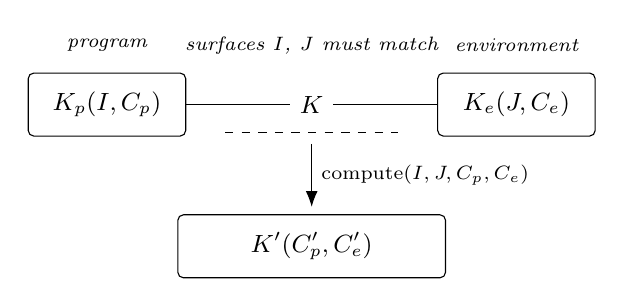
\begin{tikzpicture}[
  every node/.style={font=\small},
  box/.style={draw,rounded corners=2pt,minimum height=8mm,minimum width=20mm},
  lbl/.style={font=\scriptsize\itshape}
]
  \node[box] (kp) at (-2.6,0) {$K_p(I, C_p)$};
  \node[box] (ke) at ( 2.6,0) {$K_e(J, C_e)$};
  \node (k) at (0,0) {$K$};
  \draw (kp) -- (k); \draw (k) -- (ke);
  \node[lbl] at (-2.6,0.75) {program};
  \node[lbl] at ( 2.6,0.75) {environment};
  \draw[-{Latex[length=2mm]}] (0,-0.5) -- (0,-1.3)
        node[midway,right,font=\scriptsize] {$\compute(I,J,C_p,C_e)$};
  \node[box,minimum width=34mm] (res) at (0,-1.8) {$K'(C_p', C_e')$};
  \draw[dashed] (-1.1,-0.35) -- (1.1,-0.35);
  \node[lbl] at (0,0.75) {surfaces $I$, $J$ must match};
\end{tikzpicture}
\end{center}

We call $(\dagger)$ an \emph{interaction cut}: two introductions meet along matching
surfaces and a contraction combines their continuations. Both sides are structured ---
the eliminand is not a bare term but an introduction carrying its own continuation.

\begin{remark}[Binding is not the point]
Pseudo-application factors into two parts: the substitution $P\{u/y\}$, by which a
datum migrates from the environment continuation into the program continuation through
a binder, and the release $\mid Q$ of the environment's residual. Binding is therefore
\emph{one mode by which information migrates} under the contraction, not an intrinsic
feature of the cut. CCS realises the same shape with no migration at all, and is in this
sense the paradigmatic instance.
\end{remark}

\subsection{Surfaces: nominal and structural}
\label{subsec:surfaces}

A surface may be carried in either of two ways, and which one a calculus uses is
dictated entirely by the equational theory of $K$.

It may be carried \emph{nominally}, as an explicit $I$ or $J$ that must match --- as the
subject $x$ does in rho and $\pi$, or as complementary labels do in CCS. Or it may be
carried \emph{structurally}, by the rigidity of $K$: when $K$ is free, carrying no
equations at all, position itself is unforgeable and the context $K([\,],-)$ \emph{is}
the surface. A nominally degenerate --- absent --- surface is then not a missing match
condition but one carried by the geometry of $K$ instead.

The $\lambda$-calculus is exactly this case on the environment side. $\mathrm{App}$ is
free, and its rigidity supplies the surface that no explicit $J$ records. Each
application comprises a location together with a function and an argument; the location
is the surface, the function is the program and the argument is the environment --- or
dually. A variable, we note, is not a surface, though it is closely related to one.

The dividing line is \emph{freeness}, not commutativity. An equation on $K$ is a
congruence step: it rewrites adjacency without firing a cut. Associativity re-brackets
adjacency, a unit law inserts and deletes neighbours, idempotence copies them, and
associative--commutativity dissolves position altogether into a freely mixed soup. Each
forges position, and only a free $K$ admits no such move. We return to the consequences
in Section~\ref{subsec:capabilities}.

\subsection{Discriminating examples: three machines that are not interactive}
\label{subsec:machines}

It is easy to accumulate examples of a definition and hard to see what the definition
excludes. We therefore work three non-examples in detail. They are not exotic: they are
the machines with which most readers first learned what computation is.

\subsubsection{Turing machines}

A Turing machine is unproblematically a GSLT. Its sorts are states, tape symbols, and
configurations; its operators build a configuration from a state, a tape, and a head
position; its rewrites are the transition table together with the mechanics of moving
the head. One can write the presentation down and a machine will accept it. We do so in
Section~\ref{subsec:rubric-turing}.

What it is not is \emph{interactive} in the sense of Definition~\ref{def:igslt}. To make
it interactive one must exhibit an interaction constructor $K(P,E)$ and a $K$-headed
rule. The only plausible candidate for the site of interaction is the contact between
the finite control and the tape: that is, after all, where the machine's steps happen.
But the definition asks that $E$ be an operand of the interacting sort, and the tape is
not of the sort of the control. The candidate cut is heterogeneous, and $K(P,E)$ has no
well-sorted instance.

\begin{nonexample}[Turing machines]
\label{nonex:turing}
The Turing machine has no naive presentation as an interactive GSLT. The cut would be
between automaton and tape, which are of different kinds.
\end{nonexample}

The failure is worth dwelling on because it is not a failure of expressive power. A
Turing machine can compute anything a rho calculus term can compute. What it lacks is a
\emph{site}: a place in the syntax where two things of the same kind are brought into
contact, such that one could ask what else might have been brought into contact there
instead. The absence of such a site is precisely the absence of an environment in which
the machine could be placed --- which is another way of saying that a Turing machine is
a model of a closed computation, and interactivity is about open ones.

\subsubsection{Moore and Mealy machines}

The transducers fail in the same way and differ from each other in an instructive
second respect.

A Moore machine emits an output determined by its current state alone; a Mealy machine
emits an output determined by its current state \emph{and} the input symbol just
consumed. Both are automata reading a stream, and for both the only candidate cut is
between the machine and the stream --- again heterogeneous, again no well-sorted
$K(P,E)$. On the first axis, then, the three machines fail identically, and one might
think a single non-example would have sufficed.

It does not, because the pair discriminates along a \emph{second} axis: the migration
classification of Remark~\ref{rem:migration} below. Were one to force an interaction-cut
reading on these machines, the Moore machine's output is a function of the state alone,
so nothing of the environment reaches the emitted value; the contraction would be pure
release, the null-migration corner occupied by CCS. The Mealy machine's output depends
on the consumed symbol, so the environment's datum does reach the residual; the
contraction would migrate. Two machines that fail interactivity for the same reason
nevertheless sit at different points of the classification that organises the successes.

\begin{nonexample}[Moore and Mealy machines]
Neither transducer has a naive presentation as an interactive GSLT, for the reason of
Non-example~\ref{nonex:turing}. Under a forced reading they would occupy the
null-migration and binding-migration positions respectively.
\end{nonexample}

\subsubsection{Presentation versus encoding}

The reader will object that Turing machines can obviously be \emph{run} inside a process
calculus, and that the objection above is therefore pedantic. The objection is correct
and the distinction it presses on is the important one.

There is a difference between a theory \emph{having} a presentation and a theory
\emph{admitting an encoding into} one that does. Encoding a Turing machine into the rho
calculus --- reifying the tape as a collection of processes communicating on channels,
and the head as a process that moves among them --- produces a rho term whose behaviour
simulates the machine. That is a genuine and useful construction, and we exhibit it in
Section~\ref{subsec:rubric-turing}. But the result is a statement about rho, not about
Turing machines. The interaction sites in the encoded term are rho's sites, and the
questions one can ask of them are questions about rho contexts.

This distinction is the entire subject of Section~\ref{sec:category}, where the
morphisms of the category $\GSLT$ turn out to be exactly the well-behaved encodings, and
where the conditions under which an encoding tells you something about the source rather
than merely about the target are isolated.

%===============================================================================
\section{Continued interactive GSLTs}
\label{sec:continued}
%===============================================================================

Interactivity names a site. The constructions of Part~III need more: they need to be
able to \emph{intervene} at the site --- to interpose a token, to record an event, to
attach a guard. Three further conditions suffice, and this section isolates them.

\subsection{Section-equipped}

The first condition concerns the relationship between a term and its congruence class.
Let $T$ be the free syntax of the interacting sort and $\widehat{T} = T/{\equiv}$ its
quotient by structural congruence. Two maps relate them:

\begin{itemize}[leftmargin=2em]
  \item the \emph{quotient} $T \twoheadrightarrow \widehat{T}$, respecting $\equiv$,
    invertible up to congruence. This is the structure a name constructor exposes when
    channels are taken up to $\equiv$ --- in rho, $@P$ with $@P = @Q \iff P \equiv Q$.
  \item a \emph{section} $\cf : \widehat{T} \to T$, a choice of canonical representative
    per class.
\end{itemize}

\begin{definition}[Section-equipped]
\label{def:section}
An interactive GSLT is \textbf{section-equipped} when it comes with a computable section
$\cf : \widehat{T} \to T$ of its $\equiv$-quotient --- equivalently, a computable
canonical-form function on the interacting sort.
\end{definition}

The condition is sharper than it looks, and the $\lambda$-calculus is the test that
shows why. The $\lambda$-calculus has no analogue of the quote constructor $@$. It
passes anyway, because what is required is not a channel constructor but a section: for
$\lambda$ the congruence is $\alpha$ and a canonical representative of each
$\alpha$-class is the de Bruijn encoding~\cite{deBruijn1972}. Rho fuses the quotient and
the section into one operator viewed two ways; $\lambda$ pulls them apart; the
requirement is identical in both.

\subsection{Wrappability}

The second condition asks that the contraction tolerate having its operands decorated.
Anticipating Section~\ref{sec:cost}, write $\Tw$ for a sort of \emph{wrapped} terms.

\begin{definition}[Wrappability]
\label{def:wrappable}
The contraction $\compute$ is \textbf{wrappable} when it is well-sorted as an operation
on wrapped continuations,
$\compute : \Surf \times \Surf \times \Tw \times \Tw \to \Tw \times \Tw$ ---
equivalently, when $\compute$ is definable on decorated continuations, mapping decorated
inputs to decorated outputs.
\end{definition}

The condition is mild for substitution-like contractions: substituting a wrapped term
into a position yields a wrapped term, so $\compute$ preserves the sort for free and
need not know that wrapping exists. It excludes contractions that inspect and dismantle
their operands --- an opaque contraction returning bare residuals would violate it.

\subsection{The definition}

\begin{definition}[Continued interactive GSLT]
\label{def:cigslt}
A \textbf{continued interactive GSLT} is an interactive GSLT equipped with:
\begin{enumerate}[label=(\roman*),leftmargin=2.5em]
  \item a presentation of its dynamics in interaction-cut form $(\dagger)$, naming
    $K, K_p, K_e, K'$ and the partial contraction $\compute$;
  \item a section (Definition~\ref{def:section}); and
  \item wrappability (Definition~\ref{def:wrappable}).
\end{enumerate}
We write $\ciGSLT$ for the resulting category, whose morphisms are theory maps that are
bisimulation-preserving on the interacting sort and \emph{quote-faithful}: injective on
the reachable signature keys.
\end{definition}

The adjective names a strict strengthening. Clauses (i)--(iii) are data and conditions
added on top of an interactive GSLT, not a restriction of it; forgetting them recovers
the underlying interactive GSLT.

\begin{definition}[The forgetful functor]
$U : \ciGSLT \to \iGSLT$ sends a continued interactive GSLT to its underlying interactive
GSLT, discarding the cut presentation, the section, and the wrappability witness, and
acts as the identity on the underlying theory map of a morphism.
\end{definition}

\begin{proposition}[The distinction is proper]
\label{prop:proper}
$U$ is faithful but neither full nor essentially surjective. Hence $\ciGSLT$ is a
genuine, proper subcategory of $\iGSLT$: strictly more structure on objects, strictly
fewer morphisms between them.
\end{proposition}

\begin{proof}[Discussion]
\emph{Faithful, not full.} $U$ forgets no information about a morphism's action, so it
is faithful. It is not full because a $\ciGSLT$-morphism must additionally be
quote-faithful: an $\iGSLT$-morphism that is bisimulation-preserving yet collapses two
distinct signature keys is a map between the underlying objects with no lift.

\emph{Not essentially surjective.} Clause (i) requires the dynamics to factor as contact
then contraction, which a theory with non-local or unfactorable rewrites need not;
clause (ii) requires a computable section, which a theory with undecidable structural
congruence lacks; clause (iii) requires the contraction to preserve wrapping. An
interactive GSLT failing any of these has no preimage.
\end{proof}

\begin{remark}[$\lambda$ exhibits the distinction]
The $\lambda$-calculus is an object of $\iGSLT$ as such: terms, $\alpha$, $\beta$. It
becomes an object of $\ciGSLT$ only once one \emph{chooses} the added structure --- the
de Bruijn section for (ii), the degenerate-$K_e$ presentation of $\beta$ for (i),
substitution-on-thunks for (iii). The same underlying calculus sits at both levels,
witnessing that ``continued'' is added structure and not a property read off the
interactive GSLT alone.
\end{remark}

\subsection{How the examples are examples}
\label{subsec:table}

\begin{remark}[The migration spectrum]
\label{rem:migration}
The instances are usefully ordered by how much information the contraction moves from
the environment continuation into the program continuation. Four modes occur: no
migration (CCS, interaction categories), migration by binding (rho, $\pi$, $\lambda$),
migration by spatial restructuring (ambients), and migration as interface composition.
\end{remark}

Table~\ref{tab:cut} records the interaction-cut data of each running example, and
Table~\ref{tab:verdict} records whether that data satisfies the successive conditions.
The final column of Table~\ref{tab:verdict} is the discrimination the two strengthenings
were introduced to make.

\begin{table}[t]
\footnotesize
\centering
\begin{tabular}{@{}lllllp{34mm}@{}}
\toprule
\textbf{Instance} & \textbf{$K$} & \textbf{$E$ on $K$} & \textbf{$I$, $J$} &
\textbf{$C_p$ / $C_e$} & \textbf{$\compute$ (migration)} \\
\midrule
Calculator & --- & --- & --- & --- & no interaction rule \\[2pt]
CCS & ${\mid}$ & AC & $a$, $\bar a$ & $P$ / $Q$ &
  pure release $P \mid Q$ (none) \\[2pt]
Interaction cats. & $\circ$ & --- & shared interface & proc. / proc. &
  interface composition (none) \\[2pt]
rho, $\pi$ (sync) & ${\mid}$ & AC & $x$, $x$ & $\lambda y.P$ / $[Q_1,Q_2]$ &
  pseudo-app.\ $P\{Q_1/y\} \mid Q_2$ (binding) \\[2pt]
rho, $\pi$ (async) & ${\mid}$ & AC & $x$, $x$ & $\lambda y.P$ / $[Q,-]$ &
  pseudo-app.\ $P\{Q/y\}$ (binding) \\[2pt]
$\lambda$ & $\mathrm{App}$ & free & $x$, $-$ & $\lambda x.M$ / $N$ &
  application $M\{N/x\}$ (binding) \\[2pt]
Ambients & ${\mid}$ & AC & $n$, $n$ & $P$ / $Q$ &
  boundary dissolve/move (spatial) \\[2pt]
\midrule
Turing & \emph{none} & --- & --- & --- & control/tape heterogeneous \\[2pt]
Moore & \emph{none} & --- & --- & --- & control/stream heterogeneous \\[2pt]
Mealy & \emph{none} & --- & --- & --- & control/stream heterogeneous \\
\bottomrule
\end{tabular}
\caption{Interaction-cut data. A surface entry of $-$ denotes a nominally degenerate
surface carried structurally by the rigidity of $K$; an environment-continuation entry
of $-$ denotes a degenerate continuation, which is what distinguishes asynchronous from
synchronous output.}
\label{tab:cut}
\end{table}

\begin{table}[t]
\footnotesize
\centering
\begin{tabular}{@{}lccccl@{}}
\toprule
\textbf{Instance} & \textbf{GSLT} & \textbf{has $K$-rule} & \textbf{section $\cf$} &
\textbf{wrappable} & \textbf{Verdict} \\
\midrule
Calculator      & \checkmark & --- & normal form & --- & GSLT only \\
CCS             & \checkmark & \checkmark & normal form for AC $\mid$ & \checkmark & continued interactive \\
Interaction cats.& \checkmark & \checkmark & interface normal form & \checkmark & continued interactive \\
rho, $\pi$ (sync) & \checkmark & \checkmark & normal form for AC $\mid$ & \checkmark & continued interactive \\
rho, $\pi$ (async)& \checkmark & \checkmark & normal form for AC $\mid$ & \checkmark & continued interactive \\
$\lambda$        & \checkmark & \checkmark & de Bruijn & \checkmark & continued interactive$^\ast$ \\
Ambients         & \checkmark & \checkmark & normal form for AC $\mid$ & \checkmark & continued interactive \\
\midrule
Turing           & \checkmark & --- & --- & --- & GSLT only \\
Moore            & \checkmark & --- & --- & --- & GSLT only \\
Mealy            & \checkmark & --- & --- & --- & GSLT only \\
\bottomrule
\end{tabular}
\caption{Verdicts. $^\ast$ $\lambda$ qualifies only once the added structure is chosen;
see Remark above. The three machines are perfectly good GSLTs and fail at the first
strengthening, not the second.}
\label{tab:verdict}
\end{table}

Two readings of the tables are worth making explicit.

First, the calculator row and the three machine rows fail for \emph{different} reasons,
and the tables record the difference. The calculator has no interaction rule because it
has no notion of a program meeting an environment at all --- it is a language of closed
expressions. The machines have a notion of the control meeting something, but the
something is of the wrong sort. Both end at ``GSLT only,'' and a reader who wanted to
know which of the two situations obtains would have to look at the $K$ column.

Second, $\lambda$ is the only row whose verdict carries a caveat, and the caveat is the
content of Proposition~\ref{prop:proper}. Nothing about the $\lambda$-calculus as
ordinarily presented determines a section; de Bruijn is a choice, and a different choice
--- a different canonical form for $\alpha$-classes --- would give a different object of
$\ciGSLT$ over the same object of $\iGSLT$. This is what it means for $U$ to fail to be
essentially surjective on the nose while being surjective on the underlying calculi one
cares about.

%===============================================================================
\part*{Part II --- The category}
\addcontentsline{toc}{part}{Part II --- The category}
%===============================================================================

\section{The category \texorpdfstring{$\GSLT$}{GSLT}}
\label{sec:category}

Part~III consists of constructions that take a theory and produce a theory. To say
anything about such constructions --- that they are functorial, that they are monads,
that they have adjoints --- we need a category of theories. This section builds it, and
the build is less routine than one might expect: the obvious definition is wrong, and
the way it is wrong is instructive.

\subsection{The naive definition and three defects}

The obvious move is to take objects to be GSLTs and morphisms to be signature-preserving
translations that preserve bisimulation. Three things go wrong.

\paragraph{The constant map.} Send every term to $0$. This preserves signatures
trivially and preserves bisimulation trivially, since the image has no transitions to
fail to match. It is a morphism from anything to anything, and its presence means the
category orders nothing.

\paragraph{Milner's encoding is not a map of terms.} The canonical encoding of the
$\lambda$-calculus into the $\pi$-calculus~\cite{Milner1992} --- the very construction
that established the modern practice of comparing calculi --- sends a $\lambda$-term not
to a $\pi$-term but to a $\pi$-term \emph{parameterised by a name}: $\sem{M}_u$, the
process that realises $M$ and reports its result on $u$. Signature preservation does not
typecheck, because $\mathrm{App}$ is not sent to any single $\pi$ operator; it is sent to
a construction involving restriction, parallel composition, and output. Requiring
morphisms to be signature homomorphisms excludes the motivating example.

\paragraph{Ambient contexts observe too much.} Suppose one encodes $\pi$ into rho. A rho
context may quote a process, compare quotations, and generally observe the syntactic
form of what it is handed --- capabilities no $\pi$ context has. Bisimulation computed
over \emph{all} rho contexts will therefore separate the images of $\pi$-terms that no
$\pi$ context can separate. Under the naive definition, no interesting encoding is ever
bisimulation-preserving, for a reason that has nothing to do with the encoding.

\subsection{Contexts as the primary structure}

The three defects have one cure. The first says we need a non-degeneracy condition; the
second says terms are the wrong primitive; the third says the observer must be
restricted to what the source can express. Taking contexts rather than terms as primary
addresses all three at once, because a term is a nullary context, and because the
observers of a term are exactly the contexts one can place around it.

A theory presents a symmetric multicategory of contexts. Its objects are
\emph{interfaces}, recording the sort of a hole, its binding stage, and its interaction
surface. Its multimorphisms are contexts with holes of the given interfaces and a result
of the given interface; composition is plugging. Terms are the nullary contexts.

Transitions are then labelled by contexts: rather than $P \to P'$, we record
$P \xrightarrow{\;C\;} P'$, meaning that placing $P$ in the context $C$ enables the step.
Bisimulation is taken over these context-labelled transitions.

\begin{definition}[Morphism of theories]
\label{def:morphism}
A morphism of GSLTs is a pseudofunctor of context multicategories that is
bisimulation-preserving for context-labelled transitions, where the bisimulation on the
target is computed only over the image of the source's contexts.
\end{definition}

Each clause repairs one defect. Because the map is defined on contexts and terms are
nullary contexts, an encoding like Milner's --- which sends a term to a
context-parameterised process --- is expressible: the parameterisation is the interface.
Because bisimulation on the target is computed over the image, the ambient-observation
defect disappears by construction; the encoded $\pi$-terms are compared by the encoded
$\pi$ contexts, which is the comparison one meant to make. And the constant map is
excluded by the non-degeneracy conditions of the next subsection.

\begin{definition}[The category $\GSLT$]
\label{def:GSLTcat}
$\GSLT$ is the category whose $0$-cells are GSLTs and whose morphisms are the maps of
Definition~\ref{def:morphism}: bisimulation-preserving for the context-labelled
transition relation, which is thereby a congruence.
\end{definition}

This is the official definition for the remainder of the document. The additional
conditions imposed by particular constructions --- quote-faithfulness for the cost
functor of Section~\ref{sec:cost}, preservation of $\Pr$ and $\rsq$ for the type-system
functor of Section~\ref{sec:hypercube} --- are stated where those constructions need
them, and are refinements of Definition~\ref{def:morphism} rather than rivals to it.

\subsection{Hosting and exhausting}

Two conditions prevent the comparison from being trivial.

\begin{definition}[Hosting]
A morphism $F : G \to H$ is \emph{hosting} (faithful) when the target can run the
source: the encoding reflects as well as preserves the context-labelled transition
structure, so that no branching present in $G$ is lost in $H$.
\end{definition}

\begin{definition}[Exhausting]
$F : G \to H$ is \emph{exhausting} (dense) when the target is nothing the source cannot
assemble: every context of $H$ relevant to the image is, up to the equivalence, in the
image of a context of $G$.
\end{definition}

The constant map fails hosting immediately. Together the conditions induce a preorder on
theories whose degrees \emph{refine} Turing completeness rather than replacing it: the
classical notion is recovered as the trace collapse, obtained by coarsening
context-labelled bisimulation all the way to the input/output relation.

\begin{remark}[Why not Turing completeness]
Expressiveness comparisons between computational models are conventionally anchored to
Turing completeness. For functions this works. For interactive systems it does not,
because Turing completeness is a statement about the input/output relation, and the
input/output relation is the coarsest invariant in the linear-time/branching-time
spectrum~\cite{vanGlabbeek1990}, while the equivalences that matter for interaction sit
at the other end. Calculi of identical Turing power are routinely separated by
uniform-encoding criteria, so the yardstick is measuring something other than what is
being compared.

The obvious repair --- demand behavioural rather than computational universality ---
merely relocates the problem, since the arbiter of which behavioural equivalence to use
is an adequate modal logic, and the logical apparatus available in the ambient setting is
inherited from the $\lambda$-calculus. An absolute notion is quietly $\lambda$-relative.
Definition~\ref{def:morphism} replaces the yardstick with a relative property: fix a
probe and ask what that probe can see.
\end{remark}

\begin{remark}[A note on complexity]
The same preference for intensional over extensional comparison has a consequence for
complexity theory that we record without pursuing. Equivalence of regular languages is
\textsc{PSPACE}-complete, while the corresponding bisimulation problem is polynomial;
equivalence of context-free languages is undecidable, while the corresponding
bisimulation problem is tractable. We want the witnesses, not the extensions they give
rise to. Infinitary objects like languages cannot be grasped directly, so an intensional
representation is needed --- and once one has an intensional representation, one has a
bisimulation problem rather than a language-comparison problem.
\end{remark}

%===============================================================================
\part*{Part III --- Constructions}
\addcontentsline{toc}{part}{Part III --- Constructions}
%===============================================================================

The three sections that follow have the same shape. Each takes a theory presented as an
interaction cut and produces another such theory, decorated with apparatus. Each is a
monad. Each resolves through a free/forgetful adjunction that installs and removes the
apparatus. And in each case, when the base theory is sufficiently expressive, the
apparatus can alternatively be encoded back into the base --- so that the base performs
the metering, or the logging, or the checking, with its own computation. We note that
possibility where it arises and do not develop it.

\section{The cost monad}
\label{sec:cost}

\subsection{What is being built}

Given a continued interactive GSLT $G$, the cost endofunctor $\cost$ produces a calculus
$\cost(G)$ in which every interaction is gated on the consumption of a token. The design
question is where the gating lives, and the answer that makes the construction work is:
\emph{in the grammar of the image}.

In $\cost(G)$ the functor adjoins a sort $\Sig$ of signatures, a wrapped-term sort $\Tw$
with the wrapper $\{\cdot\}_s : P \times \Sig \to \Tw$, and a sort $\Stk$ of token stacks
\[
  S ::= (\,) \mid s :: S, \qquad s \in \Sig .
\]
The pivotal discipline is grammatical: in $\cost(G)$ every continuation slot of $K_p$ and
$K_e$ has sort $\Tw$. A continuation in the metered calculus is therefore not a bare
process awaiting metering; it is a \emph{metered thunk} $\{P\}_s$, whose activation is
gated by a token keyed to $s$, and whose own continuations are again thunks.

The signature constructor is $\# = \mathrm{digest} \circ \cf$: the section of
Definition~\ref{def:section} chooses a canonical representative, and a collision-resistant
digest commits to it. Note that $\#$ does \emph{not} respect $\equiv$, and must not,
since a commitment identifying congruent-but-distinct representatives would be no
commitment. Signatures never reduce; they are a rewrite-free sub-theory meeting the
behavioural theory only at the matching guard, so the $\equiv$-incoherence of $\#$ is
harmless for bisimulation, which factors as ``$P$-bisimulation gated by key matching.''

\subsection{The gated rules}

A wrapped redex is forced by consuming a matching token. The single-signature rule seals
the whole redex under one $s$ and funds it from a purse located at the surface
$L = \near(I,J)$:
\[
  \frac{L = \near(I,J) \qquad
        (\{C_p'\}_{t_1}, \{C_e'\}_{t_2}) = \compute(I,J,\{C_p\}_{t_1},\{C_e\}_{t_2})}
       {K\bigl(\{K(K_p(I,\{C_p\}_{t_1}), K_e(J,\{C_e\}_{t_2}))\}_s,\ S(L, s::p)\bigr)
        \longrightarrow
        K\bigl(K'(\{C_p'\}_{t_1}, \{C_e'\}_{t_2}),\ S(L,p)\bigr)}
  \tag{R1}
\]
The remaining cases seal the two interaction surfaces rather than the whole redex,
funding per surface, and are what the associative--commutative structure of $\mid$
requires when a redex is split across the bag or its tokens are supplied separately. We
write them as (R2) and (R3) and do not reproduce them here.

The decisive point is what is \emph{absent}. There is no re-wrapping step and no lifted
contraction. By the typing of $\compute$, the residual $K'(\{C_p'\}_{t_1},
\{C_e'\}_{t_2})$ is already built from wrapped terms.

\begin{definition}[Well-wrapped]
A configuration of $\cost(G)$ is \emph{well-wrapped} when it is well-sorted in the
grammar of $\cost(G)$ --- in particular, every continuation occupies a slot of sort
$\Tw$, so every redex occurrence lies inside a wrapper.
\end{definition}

\begin{lemma}[Subject reduction for wrapping]
Well-wrapping is preserved by (R1)--(R3).
\end{lemma}

\begin{proof}[Proof sketch]
Each rule replaces a wrapped redex by $K'(C_p',C_e')$ with $(C_p',C_e') = \compute(\dots)$.
Since $\compute$ lands in $\Tw \times \Tw$ and $K'$ packages terms of sort $\Tw$, the
residual is well-sorted; the consumed cell leaves a well-sorted stack; redexes elsewhere
are untouched.
\end{proof}

\begin{corollary}[No leak, by construction]
In a well-wrapped configuration no redex can fire without being unwrapped, i.e.\ without
consuming a token. There is no dynamic wrapping operation; the cost-accounting steps only
ever unwrap.
\end{corollary}

\begin{remark}[Eager versus lazy metering]
An alternative discipline re-wraps the contractum at contraction time, traversing it to
sign each exposed redex --- charging eagerly for every redex a step exposes. Wrapping by
construction charges lazily: each redex is born wrapped and is charged only when actually
forced. Lazy metering pays for work performed, not work merely exposed; redexes beneath a
discarded binder are never charged. The token stack drains exactly in step with the
reductions performed, which is also the operational reality of fuel consumption.
\end{remark}

\begin{remark}[Duplication needs no fresh signatures]
Because multiplicity is carried by the stack and not by key distinctness, copying a
wrapped term $\{Q\}_s$ copies its key but not its tokens: $n$ copies of an $s$-redex
require $n$ cells keyed to $s$. Created redexes --- where a substituted wrapped term
lands in head position --- are guarded for the same reason, since the substituted
material carries its own wrapper. One mechanism handles duplicated and created redexes
alike.
\end{remark}

\subsection{Two monoids: space and time}

The construction places two combination operators side by side, of different character.

The interaction constructor $K$ is \emph{spatial}: it records what is in contact with
what, and may carry equations --- associative--commutative in rho, free in $\lambda$.

The cons operator $::$ is \emph{temporal}: it records what is spent next, then next. It
is a free monoid, never commutative, because reduction is sequential even when
interaction is parallel. Each forcing pops a cell; the order of popping is the order of
steps. The stack is the time axis of the computation reified as a term: $\equiv$ leaves
it invariant, $\longrightarrow$ pops it, and its ordering is the arrow of the computation.

\begin{proposition}[Stack consumption is the modulus]
For a terminating reduction in $\cost(G)$, the number of cells consumed equals the number
of forced redexes, which equals the number of cuts eliminated --- including those
introduced by duplication, each charged when forced. The consumed prefix of the temporal
stack is an exact operational modulus for the cut elimination, realised by running the
reduction rather than by a separate traversal.
\end{proposition}

\subsection{The monad and its resolution}

\begin{construction}[Unit and multiplication]
Define $\eta_G(P) = \{P\}_{(\,)}$, wrapping each term with the unit signature. Since
$(\,)$ is the unit of the signature monoid, a $(\,)$-keyed redex fires without net
resource, so $\eta_G$ embeds $G$ as the cost-free fragment of $\cost(G)$. Define
$\mu_G : \cost^2(G) \to \cost(G)$ by multiplying nested signatures,
$\{\{P\}_{s_2}\}_{s_1} \mapsto \{P\}_{s_1 * s_2}$, and concatenating the stack-of-stacks
into a single stack.
\end{construction}

\begin{proposition}[The cost monad]
$(\cost, \eta, \mu)$ is a monad on $\ciGSLT$. Its laws descend from the laws of the two
constituent monoids: the unit laws from $s * (\,) = s = (\,) * s$ together with the
singleton/empty laws of the list monad, and associativity from associativity of $*$ and
of concatenation.
\end{proposition}

\begin{remark}[A genuine, non-idempotent resource monad]
$\cost$ is not idempotent: $\mu_G$ is no isomorphism, because concatenating two stacks
forgets the boundary between them and multiplying two grades forgets the factorisation.
Flattening is a true merge of two resource accounts, not the collapse of a redundant
copy. This is the expected signature of a resource monad, and it distinguishes $\cost$
from idempotent closure monads.
\end{remark}

\begin{proposition}[Free--forgetful resolution]
\label{prop:cost-adjunction}
Let $\mathrm{Cost}\text{-}\ciGSLT$ be the category of cost-accounted continued
interactive GSLTs. The functor $\mathrm{Install}$ that adjoins the apparatus is left
adjoint to the functor $\mathrm{Forget}$ that strips it, and the induced monad on
$\ciGSLT$ is $\cost$.
\end{proposition}

The embedding is structural and strict: $\mathrm{Install}$ adjoins sorts and rules,
$\mathrm{Forget}$ erases them on the nose. Crucially, forgetting is not
behaviour-preserving in the metering sense --- erasing the apparatus removes the gating,
so the forgotten theory runs its interactions without friction. The resolution answers
``what apparatus was added?'' and lets us remove it; it does not claim the metered and
un-metered dynamics agree.

\begin{remark}[Internalisation]
\label{rem:internalise-cost}
When the base theory is sufficiently expressive --- enough to code its own higher-order
syntax, whether by binding or by reflection --- the entire metering apparatus is itself
expressible in the base. Tokens become encoded data and the gated rules become an
interpreter loop, so that the base performs the metering with its own computation. This
is a second and quite different erasure from forgetting: rather than stripping the
apparatus it dissolves it into the base. We record its availability and do not develop
it here.
\end{remark}

\subsection{Capabilities and located purses}
\label{subsec:capabilities}

A cost-accounted calculus is a calculus in which the right to draw on a resource stack is
itself an authority. We must therefore ask what confers that authority, and ensure the
construction does not silently grant it. The answer turns entirely on the equational
theory of $K$, in the manner already anticipated in Section~\ref{subsec:surfaces}.

\paragraph{Free $K$: position is the capability.} When $K$ carries no equations, nothing
can drift into contact with a stack it does not already neighbour. A capability to draw
on a stack $S$ is then literally the context $K([\,], S)$ --- the right to occupy the hole
adjacent to $S$. Because $K$ is rigid, occupying that position is the whole of the
authority, and confinement is automatic. This is the $\lambda$-calculus regime and it is
the object-capability ideal: authority is structural, held by reference, and unforgeable
by construction.

\paragraph{Non-free $K$: the leak.} The moment $K$ carries any equation, position is no
longer exclusive. An equation is a congruence step that changes adjacency without firing
a cut, so it lets a program drift into contact with a stack it did not structurally
neighbour. Associative--commutativity is the limit: the bag is a freely mixed soup, every
program adjacent to every stack, and rho lives exactly here. Taking proximity as
authority in that regime is precisely \emph{ambient authority}~\cite{MillerYeeShapiro2003},
and it is a leak.

\paragraph{The repair: nominal surfaces and located stacks.} To recover an
object-capability discipline under a non-free $K$, carry the surface nominally and gate on
a nearness operator $\near(I,J)$, which when defined returns the surface at which the two
meet. Interaction is licensed not by position but by the matchability of the surfaces.
Then locate the stack at a surface,
\[
  S(I,\ s :: S') ,
\]
so that the cookie jar carries a label naming which hands may reach in. Authority over a
resource is thereby named in the term rather than conferred by the geometry of the bag.

\begin{remark}[Nearness bounds but does not eliminate competition]
$\near(I,J)$ does not by itself make access exclusive: two receivers may both be near the
same surface. What it guarantees is that only holders of a matching surface may compete
at all --- it replaces ``anyone adjacent'' with ``anyone holding a matching surface.''
Exclusivity, where required, is a matter for the type discipline of
Section~\ref{sec:hypercube}.
\end{remark}

\section{The history monad}
\label{sec:history}

\subsection{Keeping the past}

A rewrite theory that discards its past is irreversible precisely because a configuration
may have many predecessors. Recording which step was taken restores a unique one. That is
the whole idea, and packaging it gives the mirror image of Section~\ref{sec:cost}.

\begin{definition}[The history endofunctor]
$\hist$ sends a continued interactive GSLT $G$ to the theory whose configurations are
pairs of a configuration of $G$ and a word in the free monoid of rewrite events, with
each rewrite additionally appending its own event to the word.
\end{definition}

$\hist$ is the writer monad over the free monoid of rewrite events. Its unit attaches
the empty history; its multiplication concatenates.

\begin{proposition}
$(\hist, \eta, \mu)$ is a monad on $\ciGSLT$, and the evident functor installing the log
is left adjoint to the functor stripping it, with induced monad $\hist$.
\end{proposition}

\subsection{The free history is the reversible tree}

\begin{proposition}[Universal cover]
The free history makes the graph of computation paths out of a term into a \emph{tree}:
it is the universal cover of the reduction graph, and reversibility is exactly its
unique-parent property.
\end{proposition}

This is the structural content of the construction and it explains the erasures. An
erasure of history is a monad quotient, and these form a lattice between the reversible
cover and the irreversible base. The injective erasures compress the log without folding
the tree; the identifying ones fold it, closing loops so that paths revisit states. Such
an intermediate object is a quotient of the reduction graph's fundamental group by a
chosen set of loops --- an intermediate cover --- with the order-forgetting
(Mazurkiewicz) erasure folding exactly the commuting concurrent steps.

\subsection{The ledger law}

Underneath the covering-space picture sits an invariant needing no cohomology. Write
$\sigma$ for the fuel remaining and $\kappa$ for the fuel recorded as spent. Then
\[
  \sigma + \kappa = \sigma_0 ,
\]
initial fuel equals fuel remaining plus fuel recorded spent: a potential-plus-kinetic
invariant of a cost-accounted, history-keeping run. Its one-way breakage under erasure is
Landauer's principle~\cite{Landauer1961} --- the history one may erase for free is exactly
the redundant, state-recoverable part.

\subsection{The duality}

The two constructions are ledgers of the same time axis, read in opposite directions.

\begin{center}
\begin{tabular}{@{}lll@{}}
\toprule
& \textbf{Cost $\cost$} & \textbf{History $\hist$} \\
\midrule
adjoined structure & token stack & event word \\
monoid             & free (list), consumed & free (list), accumulated \\
behaviour along $\longrightarrow$ & drains & accrues \\
records            & what remains & what was spent \\
free object        & fully funded run & universal cover \\
erasure lattice    & grades of funding & subgroups of $\pi_1$ \\
physical reading   & bounded causality & recorded causality \\
\bottomrule
\end{tabular}
\end{center}

A GSLT gives causality. $\cost$ gives \emph{bounded} causality. $\hist$ gives the ability
to \emph{record} bounded causality. Running $\cost$ on an $\hist$-equipped model gives the
cost of making the recording, and the levels are worth keeping distinct rather than
collapsing: the stacking $\cost\hist\cost\hist\cdots$ is meaningful, and its fixed point
is an object of interest we do not pursue here.

\begin{remark}[Internalisation, again]
As in Remark~\ref{rem:internalise-cost}, a sufficiently expressive base theory can encode
the logging apparatus into itself, performing the record-keeping with its own
computation. The same caveat applies: this is a different erasure from forgetting, and we
note rather than develop it.
\end{remark}

\section{Generating type systems: OSLF and the Hypercube}
\label{sec:hypercube}

\subsection{OSLF as a family}

Operational Semantics in Logical Form (OSLF) is not a single algorithm but a
\emph{family} of them. Each member takes a theory presented as $(\Sigma, E, R)$ together
with a specification of a target logic, and generates from the two an assignment of
predicates to terms. The lineage runs through Hennessy--Milner
logic~\cite{HennessyMilner1985}, Stirling's modal characterisations, and, for the
reflective setting, the namespace logic of the rho calculus~\cite{MeredithRadestock2005b}.

The member we develop here is the \emph{Hypercube} algorithm of Stay, Meredith and
Wells, which generates not a modal logic for observing programs but a family of type
systems for classifying them. Both directions matter, and it is worth saying why they are
the same construction. A type is a predicate on terms; a modal formula is a predicate on
terms; the difference is bookkeeping about what one intends to do with the predicate. What
the family provides is the machinery for reading a rewrite rule as a formation rule for
predicates.

\subsection{Adequacy is not automatic}
\label{subsec:adequacy}

Because the difference between the two directions is bookkeeping, it is tempting to
suppose that anything the family generates inherits the property one wants from a
generated modal logic --- \emph{adequacy}, the characterisation of the theory's
behavioural equivalence by satisfaction. It does not, and the reason is worth stating
before the construction rather than after it.

Adequacy is a property of the \emph{target logic specification}, not of the generating
machinery. The classical Hennessy--Milner argument needs a certain minimum of logical
structure to run: something akin to a conjunction, so that a formula can record several
observations of the same state at once, and something akin to a negation, so that a
formula can record the \emph{absence} of an observation. Strip either and the argument
fails --- without negation one characterises a simulation preorder rather than
bisimulation; without conjunction one cannot separate states that differ only in how
their capabilities are bundled. A generated logic lacking either connective will fail to
have an adequacy theorem, and no amount of care in the generator repairs this, because
the deficiency is in what one asked the generator to produce.

\begin{remark}[The Hypercube functor offers no adequacy theorem]
\label{rem:no-adequacy}
The Hypercube algorithm generates a \emph{type system}, and type systems are not
generally expected to be adequate. Nobody asks of the simply-typed $\lambda$-calculus
that its typing judgement characterise observational equivalence; one asks that it be
sound, decidable, and useful. The same standard applies here. Sections~\ref{subsec:modal}
onwards should therefore be read as generating a classification discipline, not as
generating a behavioural characterisation.
\end{remark}

This is a deliberate trade, and Section~\ref{subsec:dials} describes what is bought with
it: the user dials which connectives are admitted, precisely in order to expose a surface
on which a finitely checkable fragment is generable. The cost of that expressiveness and
control is that not everything generated is necessarily adequate.

\subsection{Input: rewrites and redex positions}

The Hypercube algorithm takes as input a theory in the classifying form of
Section~\ref{subsec:classifying}. Its base rewrites have the schematic shape
\[
  x_1{:}X_1, \dots, x_n{:}X_n \ \ctxbar\ \emptyset \ \vdash\ L(\vec x) \rsq R(\vec x) ,
\]
and --- this is the crucial extra datum --- it also tracks \emph{redex positions}.
Choosing a subterm occurrence $t_j$ of $L$ with carrier $Y_j$ determines a one-hole
context $K_j[-]$ with $K_j[t_j] = L$. Write
\[
  V_j = \fv(K_j) - \fv(t_j), \qquad W_j = \fv(t_j) - \fv(K_j) .
\]
The variables in $V_j$ --- free in the context but not in the chosen subterm --- become
the \emph{rely parameters} of the modality generated at that position.

\begin{remark}[The relationship to the interaction cut]
The reader will recognise $K_j$. In a theory presented as an interaction cut, the contact
site $K$ of $(\dagger)$ \emph{is} a one-hole context in exactly this sense, and the
distinguished positions are the two introductions. The interaction cut is thus the
special case in which one privileges a particular family of redex positions, and the
Hypercube algorithm is what one gets by not privileging them. This is why
Section~\ref{sec:interactive} does real work for the present section: it identifies which
positions are canonical.
\end{remark}

\subsection{The modal layer}
\label{subsec:modal}

For each base rewrite and each chosen redex position, the algorithm introduces a primitive
modality
\[
  \angles{K_j}{\vec x :: \vec A}{B} ,
\]
a type former at carrier $Y_j$, read as a \emph{rely-possibly} specification: under the
rely assumptions $\vec x :: \vec A$, placing a term into the context $K_j[-]$ takes one
step to a specified right-hand side inhabiting $B$.

\begin{mathpar}
\inferrule*[right=M-Form]
  { \bigl(\Gamma \ctxbar \Delta \vdash A_k :: s_k^{X_k}\bigr)_{x_k \in V_j} \\
    \Gamma, \vec x{:}\vec X \ctxbar \Delta, \vec x{::}\vec A \vdash B :: s_{\mathrm{out}}^{\Pr} }
  { \Gamma \ctxbar \Delta \vdash \angles{K_j}{\vec x :: \vec A}{B} :: s_{\mathrm{out}}^{Y_j} }
\end{mathpar}

\begin{mathpar}
\inferrule*[right=M-Intro]
  { \bigl(\Gamma \ctxbar \Delta \vdash A_k :: s_k^{X_k}\bigr)_{x_k \in V_j} \\
    \Gamma, \vec w{:}\vec W, \vec x{:}\vec X \ctxbar \Delta, \vec x{::}\vec A \vdash B :: s_{\mathrm{out}}^{\Pr} \\
    \Gamma, \vec w{:}\vec W, \vec x{:}\vec X \ctxbar \Delta, \vec x{::}\vec A \vdash R(\vec x, \vec w) :: B }
  { \Gamma, \vec w{:}\vec W \ctxbar \Delta \vdash t_j(\vec w) :: \angles{K_j}{\vec x :: \vec A}{B} }
\end{mathpar}

Elimination is where a rewrite-generated modality differs from an equation-generated one.
Because the modality comes from a \emph{rewrite}, elimination does not provide full
conversion; it provides the operational step to the specified right-hand side, and the
typing of that right-hand side.

\begin{mathpar}
\inferrule*[right=M-Step]
  { \Gamma \ctxbar \Delta \vdash t :: \angles{K_j}{\vec x :: \vec A}{B} \\
    \bigl(\Gamma \ctxbar \Delta \vdash u_k :: A_k\bigr)_{x_k \in V_j} }
  { \Gamma \ctxbar \Delta \vdash K_j[t][\vec u/\vec x] \rsq R(\vec u) }
\and
\inferrule*[right=M-Elim]
  { \Gamma \ctxbar \Delta \vdash t :: \angles{K_j}{\vec x :: \vec A}{B} \\
    \bigl(\Gamma \ctxbar \Delta \vdash u_k :: A_k\bigr)_{x_k \in V_j} }
  { \Gamma \ctxbar \Delta \vdash R(\vec u) :: B[\vec u/\vec x] }
\end{mathpar}

To recover a conversion-like principle stable under rewriting, the algorithm freely adds
an \emph{empty-context possibility} operator $\Diamond$ at the carrier of programs, with
$p :: \Diamond B$ asserting that $p$ can take one step to some reduct of type $B$.
Equation-generated modalities, by contrast, do support full conversion by the usual rule ---
they are ``zero-step'' steps.

\subsection{The structural and propositional layers}

The modal fragment is intentionally behavioural, and this has a consequence that should
be stated plainly rather than discovered: \emph{terms with no available one-step behaviour
need not have any modal type at all.} A value, a normal form, a deadlocked process ---
none of these is classified by a layer whose formation rules are indexed by rewrites.

Two further layers repair this and extend expressivity.

\paragraph{Structural types.} For each term former $f$ the algorithm freely adds a type
former $f^\sharp$ whose inhabitants are exactly those terms whose root former is $f$.
These classify by the root of the parse tree, giving a baseline typing for programs which
can then be combined with the modal layer to express shape and one-step behaviour in the
same language. When the interaction constructor is read this way it becomes a
separating-style connective: a term satisfies $K(\varphi_1,\varphi_2)$ when it splits
across $K$ into a part satisfying $\varphi_1$ and a part satisfying $\varphi_2$. When $K$
is associative--commutative this is a genuine separating conjunction in the sense of
spatial and separation logics~\cite{CairesCardelli2003,Reynolds2002}; when $K$ is free it
is a positional split.

\paragraph{Propositional operations, stratified.} At each carrier and sort the algorithm
adds propositional operations on type formers --- but \emph{stratified by the categorical
strength required to interpret them}. The finite-limits fragment supplies $\top$ and
$\wedge$. Additional structure is required for $\bot$, for finite joins and
distributivity, and finally for implication and negation.

\begin{remark}[What a specification must supply]
\label{rem:stratification}
The stratification is not a technicality of the metatheory; it is visible to the user of
a generated logic. A specification whose classifying theory has finite limits and no more
yields a conjunctive fragment; implication and negation become available only when the
theory supplies the structure to interpret them. A developer writing a property is
therefore working in a logic whose connectives are determined by their own specification,
and a property that fails to elaborate may be failing for this reason rather than because
it is false.
\end{remark}

\subsection{Sort slots and the equational centre}

Why a \emph{hypercube}? Each generated type former carries finitely many sort slots: one
for each rely input and one for the output. Filling each slot with $\ast$ or $\Box$ yields
a raw Boolean cube of choices. But equational axioms and rewrite laws force certain slots
to agree, and only the assignments stable under those laws survive. These form the
\emph{equational centre} $\Zc$, and the vertices of the resulting hypercube are the
elements of $\Zc$.

The cube's axes are not postulated. They are determined locally by the free variables of
operational contexts and the result types demanded by the rules.

\subsection{Worked example: a rho-calculus modality}
\label{subsec:rho-modality}

Fix arity $1$. The communication rewrite is
\[
  n{:}\Nm,\ p{:}\Pr,\ \lambda x.q : [\Nm \to \Pr] \ \ctxbar\ \emptyset \ \vdash\
  \mathsf{out}_1(n,p) \mid \mathsf{in}_1(n, \lambda x.q) \ \rsq\ q[@p/x] .
\]
Choose the continuation redex position
\[
  t_j := \lambda x.q, \qquad K_j([-]) := \mathsf{out}_1(n,p) \mid \mathsf{in}_1(n,[-]) ,
\]
so that $K_j[t_j]$ is the left-hand side. The free variables of $K_j$ are
$V_j = \{n,p\}$, hence the induced modality is $\angles{K_j}{n :: A_n,\ p :: A_p}{B}$ at
carrier $[\Nm \to \Pr]$, contributing three local sort slots
\[
  \{\, s_n^{\Nm},\ s_p^{\Pr},\ s_{\mathrm{out}} \,\} .
\]
Relative to the origin assignment $(\ast,\ast,\ast)$, every nonempty subset of the three
slots can be lifted to $\Box$, yielding $2^3 - 1 = 7$ local axes.

Now hold $s_n = \ast$ fixed. Operationally the channel $n$ serves only to ensure that the
input and output are co-addressed; the reduct $q[@p/x]$ does not otherwise depend on it.
The remaining two-slot subgeometry is:

\begin{center}
\begin{tabular}{@{}lcc@{}}
\toprule
\textbf{Vertex (at $s_n = \ast$)} & $s_p^{\Pr}$ & $s_{\mathrm{out}}$ \\
\midrule
simply-typed corner        & $\ast$ & $\ast$ \\
polymorphism direction     & $\Box$ & $\ast$ \\
dependent-types direction  & $\ast$ & $\Box$ \\
type-constructors direction& $\Box$ & $\Box$ \\
\bottomrule
\end{tabular}
\end{center}

This is Barendregt's square~\cite{Barendregt1991}, recovered exactly. The three nontrivial
directions correspond to the three extra edges of the Lambda Cube beyond the simply-typed
corner. \emph{The Cube is one face of one modality of one rewrite rule.} It arises here
not because it was postulated but because the communication rule has two rely parameters
and one output, and the sort slots of a two-parameter modality form a square.

\begin{remark}[Why Barendregt needed no equational centre]
In the Lambda Cube there are no built-in equations, and the underlying equations of
$\beta$ add no relations between sorts. The whole raw Boolean cube is therefore
admissible, $\Zc$ is everything, and the distinction between the raw cube and the centre
never arises. It arises for us as soon as a specification carries equations --- which, by
rung two of the ladder, is essentially always.
\end{remark}

\subsection{The construction is a monad}

Let $\Lcat$ denote the category of theories in classifying form, with morphisms preserving
$\Pr$, $\rsq$, and the internal-language structure, and let $\Lcat_\Sigma$ denote the
category of such theories equipped with the additional structure provided by the modal,
structural, and propositional layers. On a morphism $F$, the action is by transport:
\[
  \angles{K_j}{\vec x :: \vec A}{B} \ \longmapsto\
  \angles{F(K_j)}{\vec x :: F(\vec A)}{F \cdot B} ,
  \qquad \Diamond B \longmapsto \Diamond (F \cdot B) .
\]

\begin{proposition}
There is a forgetful functor $U : \Lcat_\Sigma \to \Lcat$ and a left adjoint
$F : \Lcat \to \Lcat_\Sigma$ freely adjoining the layers, and the induced endofunctor
\[
  \hyp \;=\; U \circ F \;:\; \Lcat \longrightarrow \Lcat
\]
is a monad on $\Lcat$: for each theory $\mathsf{T}$, $\hyp(\mathsf{T})$ is the underlying
theory of its free extension by generated type formers.
\end{proposition}

This completes the pattern of Part~III. Three constructions, three monads, three
free/forgetful resolutions:
\[
  \cost \ \text{(meter it)}, \qquad
  \hist \ \text{(log it)}, \qquad
  \hyp  \ \text{(type it)} .
\]
In each case the left adjoint installs apparatus generated from the theory's own
presentation, and the right adjoint takes it away.

\subsection{Three dials}
\label{subsec:dials}

Section~\ref{subsec:adequacy} said that adequacy is a property of the target logic
specification. This subsection is the other half of that statement: the target logic
specification is something the \emph{user} supplies, and supplying it is the design
activity around which the whole apparatus is arranged.

Because the logic is generated from a language specification together with a choice of
connectives, a user can select \emph{fragments} to dial in finitely checkable properties.
There are three axes:

\begin{enumerate}[label=(\arabic*),leftmargin=2.5em]
  \item \textbf{The language fragment.} Restrict the sub-signature over which properties
    are stated. A property quantifying over a decidable fragment of the terms is a
    different proposition from the same property over the whole theory.
  \item \textbf{The connective fragment.} Restrict which of the generated connectives are
    in play, subject to Remark~\ref{rem:stratification}. The conjunctive--modal fragment
    behaves very differently from one closed under negation and implication.
  \item \textbf{The cube vertex.} Choose an element of the equational centre $\Zc$. This
    is the classical design choice --- how much dependency to admit --- now presented as a
    coordinate rather than a fork in the literature.
\end{enumerate}

Each axis trades expressivity for checkability, and the three are independent. In the
general case, where the user has chosen not to constrain things statically, an
\emph{inference token budget} prevents runaway property checks. The budget is the backstop,
not the primary mechanism: the primary mechanism is fragment selection, and the budget
catches what selection did not.

\begin{remark}[Adequacy and checkability pull against each other]
\label{rem:tension}
It would be convenient if the dials traded a property nobody wanted for one everybody did.
They do not, and the tension is structural rather than incidental. Adequacy requires
negation (Section~\ref{subsec:adequacy}); negation is among the first connectives a user
drops when chasing decidability, since it is what turns a search for a witness into a
search over all possible witnesses. A user who dials down to a finitely checkable fragment
has, in the typical case, dialled out of the adequate region on the way.

The right conclusion is not that one of the two properties is illusory but that they
answer different questions. Adequacy asks whether the logic can \emph{distinguish} exactly
the programs the theory distinguishes --- a question about the logic's resolving power as a
whole. Checkability asks whether a particular property can be decided of a particular
program in bounded time. A user guarding a communication in Section~\ref{subsec:where}
wants the second and has no use for the first. A user reasoning about when two
implementations may be substituted wants the first and will accept a semi-decision
procedure for it. The dials exist so that neither user has to pay for the other's
requirement.
\end{remark}

%===============================================================================
\part*{Part IV --- Implementation}
\addcontentsline{toc}{part}{Part IV --- Implementation}
%===============================================================================

\section{Rholang 1.4: a DDL whose data can wiggle}
\label{sec:rholang}

\subsection{Two sublanguages}

Most languages have two sublanguages: a \emph{data definition language} (DDL), in which
one says what values there are, and a \emph{control flow language} (CFL), in which one
says what happens, when, and under what conditions. Rholang~1.4 has both, and the interest
of the arrangement lies in what each of them turns out to be.

The three clauses of that gloss are not decoration; each is carried by a distinct piece of
syntax, and Section~\ref{subsec:where} takes them in turn. \emph{What} happens is the
continuation. \emph{When} is the join-and-sequence structure of the
\texttt{for}-comprehension --- which receives must occur together, and which groups
follow which. \emph{Under what conditions} is the guard.

The DDL is the \texttt{language!} block. It has a superpower: \emph{the data can wiggle}.
The reader has already seen why. A \texttt{language!} specification is exactly the triple
of Definition~\ref{def:gslt}, and the ladder of Section~\ref{subsec:ladder} is its
expressivity story:

\begin{center}
\begin{tabular}{@{}lll@{}}
\toprule
\textbf{Blocks populated} & \textbf{What is presentable} & \textbf{Familiar name} \\
\midrule
\texttt{types}, \texttt{terms} & free term algebras & algebraic data types \\
$+$ \texttt{equations} & quotients of free algebras & finitely presentable universal algebra \\
$+$ \texttt{rewrites} & theories with dynamics & domain-specific languages \\
\bottomrule
\end{tabular}
\end{center}

An ordinary DDL stops at the first row. Adding equations reaches the second, which is
where a good many libraries secretly live --- every time a developer documents that a
data structure is ``a list but order doesn't matter'' or ``a string but compared
case-insensitively,'' they are hand-maintaining an equational presentation their type
system cannot see. Adding rewrites reaches the third, and at that point the DDL is
defining languages.

The CFL is merely a Rholang in which the channels are typed by \texttt{language!}
specifications. That is the whole design. A channel's type is a GSLT; sending on a channel
means sending a term of that theory; and --- because the theory comes with a generated
logic by Section~\ref{sec:hypercube} --- receiving on a channel can be guarded by a
property expressed in that theory's own logic.

\subsection{The \texttt{for}-comprehension and its guard}
\label{subsec:where}

The \texttt{for}-comprehension has grown a clause. Its generic form is
\begin{lstlisting}
for( ptrn_11 <- chan_11 & ... & ptrn_m1 <- chan_m1 ;
     ...                                           ;
     ptrn_1n <- chan_1n & ... & ptrn_mn <- chan_mn
     where condition ) P
\end{lstlisting}
where \texttt{\&} joins within a group --- simultaneity, all of the joined receives
occurring together --- and \texttt{;} separates groups. The new clause is
\texttt{where condition}, which gates the communication: the comm fires only if the
condition holds. The preceding clauses bind variables, and those variables may be
mentioned in the condition, so the guard is a condition on what was actually received.

The condition grammar is
\[
\begin{array}{rcl}
\varphi, \psi &::=& \mathtt{true} \ \mid\ \mathtt{false} \\
  &\mid& \textit{ground formula from a language definition} \\
  &\mid& \mathord{\sim}\varphi \ \mid\ \varphi \mathbin{\&} \psi
        \ \mid\ \varphi \mathbin{\backslash/} \psi
        \ \mid\ \varphi \Rightarrow \psi \\
  &\mid& \textit{spatial connectives from a language definition} \\
  &\mid& \langle K \rangle \varphi
\end{array}
\]

Every clause of that grammar has been constructed in Part~III. The ground formulae and the
spatial connectives are supplied by the language definition, which is to say by the
structural layer of Section~\ref{sec:hypercube} --- one ground formula per term former, and
the interaction constructor read separating-style. The boolean connectives are the
propositional layer, subject to the stratification of Remark~\ref{rem:stratification}. And
$\langle K \rangle \varphi$ is the modal layer.

\begin{remark}[One $K$, three altitudes]
\label{rem:oneK}
The $K$ in $\langle K \rangle \varphi$ is not a new notion. It is the same object at three
altitudes of the development. In Section~\ref{sec:category} it labels transitions, and
bisimulation --- hence the identity of programs --- is computed over context-labelled
steps. In Section~\ref{sec:hypercube} it indexes the generated modality
$\angles{K_j}{\vec x :: \vec A}{B}$, arising from a rewrite together with a choice of redex
position. Here it is what a developer types in a \texttt{where} clause. The mathematical
apparatus that makes the category work, the logic generated from a specification, and the
surface syntax of a guard are three presentations of one thing.
\end{remark}

\begin{remark}[Budgets, and what a guard is for]
Evaluating a guard is work performed at communication time, before the comm commits, and
it is metered. Token budgets rein in infinitary computations and property checks alike;
in the terms of Section~\ref{subsec:dials}, a user who has selected a finitely checkable
fragment does not rely on the budget, and a user who has not is caught by it.

It is worth being explicit that the logic a guard is written in need not be adequate, and
that this is not a compromise. A \texttt{where} clause asks whether \emph{this} received
term has \emph{that} property, in bounded time. It does not ask the logic to resolve the
theory's behavioural equivalence. By Remark~\ref{rem:tension} the two demands pull in
opposite directions, and the guard is squarely on the checkability side of that tension.
\end{remark}

\subsection{The rubric}

The remainder of this section works one pattern four times. For each of four theories we

\begin{enumerate}[label=(\arabic*),leftmargin=2.5em]
  \item define the GSLT as a \texttt{language!} specification;
  \item make an instance of a program in that GSLT and send it on a channel; and
  \item receive the program on a channel and check it for a property.
\end{enumerate}

The theories are the $\lambda$-calculus, Turing machines, the $\pi$-calculus, and the
ambient calculus. They are chosen to span the discriminations of Part~I: $\lambda$ has a
free $K$ and a degenerate environment surface; Turing machines are a GSLT and nothing more;
$\pi$ migrates by binding; ambients migrate by spatial restructuring.

\subsubsection{The \texorpdfstring{$\lambda$}{lambda}-calculus}

\begin{lstlisting}
language! {
    name: Lambda,
    types { Term },
    terms {
        Lam . ^x.body:[Term -> Term] |- "lam " x "." body : Term;
        App . fun:Term, arg:Term     |- "(" fun "," arg ")" : Term;
    },
    equations { },
    rewrites {
        Beta     . |- (App (Lam fun) arg) ~> (eval fun arg);
        AppCongL . | M0 ~> M1 |- (App M0 N) ~> (App M1 N);
        AppCongR . | N0 ~> N1 |- (App M N0) ~> (App M N1);
        LamCong  . | S ~> T   |- (Lam ^x.S) ~> (Lam ^x.T);
    },
}
\end{lstlisting}

Send a term --- here the self-application combinator applied to the identity:

\begin{lstlisting}
new work in {
  work!( (lam x . (x , x) , lam y . y) )
}
\end{lstlisting}

Receive it and guard on a property. The property we want is ``this term can take a
$\beta$-step'' --- that is, the modality generated by the \texttt{Beta} rewrite at the
top-level redex position:

\begin{lstlisting}
for( t <- work where <Beta> true ) {
  // t is a Lambda term that has a beta-redex at the root
  reduce!(*t)
}
\end{lstlisting}

\subsubsection{Turing machines}
\label{subsec:rubric-turing}

Section~\ref{subsec:machines} argued that a Turing machine is a GSLT and not an interactive
one. Both halves of that claim are visible here. The specification is unproblematic:

\begin{lstlisting}
language! {
    name: Turing,

    types {
        Config
        Tape
        State
        Sym
    },

    terms {
        Blank . Sym  ::= "_" ;
        Zero  . Sym  ::= "0" ;
        One   . Sym  ::= "1" ;

        Halt  . State ::= "halt" ;
        Q     . n:UInt32 |- "q" n : State ;

        // tape as a zipper: reversed left context, head symbol, right context
        Tp    . l:List(Sym), h:Sym, r:List(Sym) |- "<" l "|" h "|" r ">" : Tape ;

        Cf    . q:State, t:Tape |- "(" q "," t ")" : Config ;
    },

    equations { },

    rewrites {
        // one entry of the transition table, written out
        // q0 reading 0: write 1, move right, go to q1
        D_q0_0 . |- (Cf (Q 0u32) (Tp L Zero R))
                    ~> (Cf (Q 1u32) (shift_right L One R));
        D_q0_1 . |- (Cf (Q 0u32) (Tp L One R))
                    ~> (Cf Halt (Tp L One R));
    },
}
\end{lstlisting}

What one cannot write is an interaction constructor. There is no term former $K$ taking a
\texttt{Config} and an environment of the same sort into contact, because the only thing
a configuration meets is its own tape --- and \texttt{Tape} is not \texttt{Config}. The
specification is accepted, the machine runs, and the theory sits at ``GSLT only'' in
Table~\ref{tab:verdict}.

Sending and guarding nevertheless work, because they are operations of the CFL, not of the
theory:

\begin{lstlisting}
new work in {
  work!( (q0 , <[] | 0 | [0,1]>) )
  |
  for( c <- work where <D_q0_0> true ) {
    // c is a Config whose next step is the write-1-move-right transition
    step!(*c)
  }
}
\end{lstlisting}

This is the presentation/encoding distinction of Section~\ref{subsec:machines} made
concrete. The channel \texttt{work} is a Rholang channel; the interaction happens at
Rholang's cut, not at any cut of the Turing theory. What the guard inspects is a
\texttt{Turing} term; what does the inspecting is a rho comm.

\subsubsection{The \texorpdfstring{$\pi$}{pi}-calculus}

\begin{lstlisting}
language! {
    name: Pi,

    types { Proc  Name },

    terms {
        PZero . Proc ::= "0" ;
        PNew  . ^x.p:[Name -> Proc] |- "new" "(" x "," p ")" : Proc ;
        PIn   . n:Name, ^x.p:[Name -> Proc] |- n "?" x "." p : Proc ;
        POut  . n:Name, m:Name, p:Proc |- n "!" m "." p : Proc ;
        PPar  . ps:HashBag(Proc) |- "{" ps.*sep("|") "}" : Proc ;
        PRep  . p:Proc |- "!" p : Proc ;
    },

    equations {
        NewComm  . |- (PNew ^x.(PNew ^y.P)) = (PNew ^y.(PNew ^x.P)) ;
        ScopeExt . | x # ...rest
                 |- (PPar {(PNew ^x.P), ...rest}) = (PNew ^x.(PPar {P, ...rest})) ;
        RepUnfold . |- (PRep P) = (PPar {P, (PRep P)}) ;
    },

    rewrites {
        Comm . |- (PPar {(PIn n ^x.p), (POut n m q), ...rest})
                  ~> (PPar {(subst ^x.p m), q, ...rest}) ;

        ParCong . | S ~> T |- (PPar {S, ...rest}) ~> (PPar {T, ...rest}) ;
        NewCong . | S ~> T |- (PNew ^x.S) ~> (PNew ^x.T) ;
    },
}
\end{lstlisting}

The interaction-cut data is legible directly from the \texttt{Comm} rule: $K$ is
\texttt{PPar}, whose \texttt{HashBag} carrier makes it associative--commutative; the
introductions are \texttt{PIn} and \texttt{POut}; the surfaces are the subjects $n$,
matched by name equality; the continuations are $\lambda x.p$ and $(m,q)$; and the
contraction is pseudo-application, migrating $m$ into $p$ through the binder $x$.

Send a $\pi$-term and guard on a spatial property --- here, that the received process
splits into a part that can communicate and an arbitrary remainder:

\begin{lstlisting}
new work in {
  work!( new(c, { c?y.0 | c!c.0 }) )
  |
  for( p <- work where PPar( <Comm> true , true ) ) {
    schedule!(*p)
  }
}
\end{lstlisting}

The connective \texttt{PPar(-,-)} is the structural type former generated from the term
former \texttt{PPar}, read separating-style; because \texttt{PPar} is
associative--commutative, it is a genuine separating conjunction.

\subsubsection{The ambient calculus}

\begin{lstlisting}
language! {
    name: Ambient,
    types { Proc  Name },
    terms {
        PZero . Proc ::= "0" ;
        PIn   . Proc ::= "in(" Name "," Proc ")" ;
        POut  . Proc ::= "out(" Name "," Proc ")" ;
        POpen . Proc ::= "open(" Name "," Proc ")" ;
        PAmb  . Proc ::= Name "[" Proc "]" ;
        PNew  . ^x.p:[Name -> Proc] |- "new" "(" x "," p ")" : Proc ;
        PPar  . Proc ::= HashBag(Proc) sep "|" delim "{" "}" ;
    },
    equations {
        NewComm  . |- (PNew ^x.(PNew ^y.P)) = (PNew ^y.(PNew ^x.P)) ;
        ScopeExt . | x # ...rest
                 |- (PPar {(PNew ^x.P), ...rest}) = (PNew ^x.(PPar {P, ...rest})) ;
        AmbNew   . | x # P |- (PAmb N (PNew ^x.P)) = (PNew ^x.(PAmb N P)) ;
    },
    rewrites {
        InRule . |- (PPar {(PAmb N (PPar {(PIn M P), ...rest1})), (PAmb M R), ...rest2})
                   ~> (PPar {(PAmb M (PPar {(PAmb N (PPar {P, ...rest1})), R})), ...rest2}) ;

        OutRule . |- (PAmb M (PPar {(PAmb N (PPar {(POut M P), ...rest1})), R, ...rest2}))
                   ~> (PPar {(PAmb N (PPar {P, ...rest1})), (PAmb M R), ...rest2}) ;

        OpenRule . |- (PPar {(POpen N P), (PAmb N Q), ...rest})
                   ~> (PPar {P, Q, ...rest}) ;

        ParCong . | S ~> T |- (PPar {S, ...rest}) ~> (PPar {T, ...rest}) ;
        AmbCong . | S ~> T |- (PAmb N S) ~> (PAmb N T) ;
        NewCong . | S ~> T |- (PNew ^x.S) ~> (PNew ^x.T) ;
    },
}
\end{lstlisting}

This is the instance in which the contraction is neither a release nor a substitution.
\texttt{OpenRule} dissolves the boundary of an ambient, releasing its contents into the
enclosing context; \texttt{InRule} and \texttt{OutRule} relocate a subtree across a
boundary. In every case $\compute$ is a spatial restructuring: no datum migrates through a
binder, yet the configuration's nesting --- and hence what is near what --- is rearranged.
The ambient calculus is therefore the cleanest instance in which the contraction is a tree
rewrite, and its presentation in the style of Cardelli and Gordon is what
Section~\ref{sec:gslt} was pointing at.

Send an ambient term and guard on its capacity to dissolve a boundary:

\begin{lstlisting}
new work in {
  work!( { open(n, 0) | n[ m[0] ] } )
  |
  for( a <- work where <OpenRule> true ) {
    unpack!(*a)
  }
}
\end{lstlisting}

%===============================================================================
\section{Conclusion}
%===============================================================================

The through-line of this document is a single claim about where effort belongs. A
language presented as $(\Sigma, E, R)$ is not merely documented by its presentation; it is
\emph{determined} by it, in a strong enough sense that the artifacts one normally builds
by hand become instances of constructions that do not know which language they are applied
to.

Part~I isolated the structure those constructions require, and isolated it in stages so
that the requirements could be seen separately. A bare GSLT is a rewrite theory. An
interactive GSLT additionally names a site --- and the three machines of
Section~\ref{subsec:machines} are in the document precisely because they show that naming
a site is a real condition, failed by theories no one would call impoverished. A continued
interactive GSLT presents the site as a cut, supplies a canonical form, and tolerates
decoration of its continuations.

Part~II built the category, and the build was not routine: contexts, not terms, are the
primary structure, because the canonical encodings are not maps of terms and because
ambient contexts in a richer theory observe more than the encoded contexts of a poorer
one.

Part~III exhibited three constructions on that category, all of the same shape ---
$\cost$ meters, $\hist$ logs, $\hyp$ types. Each is a monad, each resolves through a
free/forgetful adjunction, and each, over a sufficiently expressive base, can alternatively
be dissolved into the base's own computation.

Part~IV closed the loop. The \texttt{language!} block is a data definition language whose
three rungs are exactly the three components of Definition~\ref{def:gslt}, and the control
flow language is a Rholang whose channels carry those specifications as types. The
\texttt{where} clause is where the parts meet: a guard written in the logic generated from
the channel's own type, over the modality $\langle K \rangle \varphi$ whose $K$ is the same
$K$ that labels the transitions over which program identity is decided.

\subsection*{Open threads}

Three, recorded for the reader who wants to push.

\emph{The stacking.} $\cost$ and $\hist$ compose, and the composite has a reading: running
$\cost$ on an $\hist$-equipped model gives the cost of making the recording. The tower
$\cost\hist\cost\hist\cdots$ and its fixed point are objects we have not investigated.

\emph{Budget semantics.} A guard whose evaluation exhausts its inference budget must do
\emph{something}, and the choices --- evaluate to false, block, fault --- are behaviourally
distinct and therefore visible to the bisimulation of Section~\ref{sec:category}. Negation
over a truncated check is where the choice bites hardest. This document specifies the
budget and not the semantics of its exhaustion.

\emph{Self-hosting.} The rho calculus is presentable as a \texttt{language!} specification;
the CFL is a Rholang. The DDL can therefore define the CFL, and the strength of the
resulting self-hosting claim --- and what it would take to make it precise --- is left
open here.

%===============================================================================
\begin{thebibliography}{99}

\bibitem{AbramskyGayNagarajan1996}
S.~Abramsky, S.~Gay, and R.~Nagarajan.
\newblock Interaction categories and the foundations of typed concurrent programming.
\newblock In \emph{Deductive Program Design}, Springer, 1996.

\bibitem{BaezWilliams2020}
J.~Baez and C.~Williams.
\newblock Enriched Lawvere theories for operational semantics.
\newblock \emph{Electronic Proceedings in Theoretical Computer Science}, 2020.

\bibitem{Barendregt1991}
H.~Barendregt.
\newblock Introduction to generalized type systems.
\newblock \emph{Journal of Functional Programming}, 1(2):125--154, 1991.

\bibitem{CairesCardelli2003}
L.~Caires and L.~Cardelli.
\newblock A spatial logic for concurrency (part I).
\newblock \emph{Information and Computation}, 186(2):194--235, 2003.

\bibitem{CardelliGordon2000}
L.~Cardelli and A.~D.~Gordon.
\newblock Mobile ambients.
\newblock \emph{Theoretical Computer Science}, 240(1):177--213, 2000.

\bibitem{deBruijn1972}
N.~G.~de~Bruijn.
\newblock Lambda calculus notation with nameless dummies.
\newblock \emph{Indagationes Mathematicae}, 34:381--392, 1972.

\bibitem{HennessyMilner1985}
M.~Hennessy and R.~Milner.
\newblock Algebraic laws for nondeterminism and concurrency.
\newblock \emph{Journal of the ACM}, 32(1):137--161, 1985.

\bibitem{LambekScott1986}
J.~Lambek and P.~J.~Scott.
\newblock \emph{Introduction to Higher Order Categorical Logic}.
\newblock Cambridge University Press, 1986.

\bibitem{Landauer1961}
R.~Landauer.
\newblock Irreversibility and heat generation in the computing process.
\newblock \emph{IBM Journal of Research and Development}, 5(3):183--191, 1961.

\bibitem{Lawvere1963}
F.~W.~Lawvere.
\newblock Functorial semantics of algebraic theories.
\newblock PhD thesis, Columbia University, 1963.

\bibitem{MeredithRadestock2005}
L.~G.~Meredith and M.~Radestock.
\newblock A reflective higher-order calculus.
\newblock \emph{Electronic Notes in Theoretical Computer Science}, 141(5):49--67, 2005.

\bibitem{MeredithRadestock2005b}
L.~G.~Meredith and M.~Radestock.
\newblock Namespace logic: a logic for a reflective higher-order calculus.
\newblock In \emph{Trustworthy Global Computing}, Springer, 2005.

\bibitem{MillerYeeShapiro2003}
M.~S.~Miller, K.-P.~Yee, and J.~Shapiro.
\newblock Capability myths demolished.
\newblock Technical report, Johns Hopkins University, 2003.

\bibitem{Milner1989}
R.~Milner.
\newblock \emph{Communication and Concurrency}.
\newblock Prentice Hall, 1989.

\bibitem{Milner1992}
R.~Milner.
\newblock Functions as processes.
\newblock \emph{Mathematical Structures in Computer Science}, 2(2):119--141, 1992.

\bibitem{Plotkin1981}
G.~D.~Plotkin.
\newblock A structural approach to operational semantics.
\newblock Technical Report DAIMI FN-19, Aarhus University, 1981.

\bibitem{Plotkin2004}
G.~D.~Plotkin.
\newblock The origins of structural operational semantics.
\newblock \emph{Journal of Logic and Algebraic Programming}, 60--61:3--15, 2004.

\bibitem{Reynolds2002}
J.~C.~Reynolds.
\newblock Separation logic: a logic for shared mutable data structures.
\newblock In \emph{LICS}, 2002.

\bibitem{StayMeredith2016}
M.~Stay and L.~G.~Meredith.
\newblock Higher category models of the pi-calculus.
\newblock arXiv:1504.04311, 2016.

\bibitem{vanGlabbeek1990}
R.~J.~van~Glabbeek.
\newblock The linear time--branching time spectrum.
\newblock In \emph{CONCUR}, Springer, 1990.

\end{thebibliography}

\end{document}
